\chapter{Solutions to Deterministic Burger's Equation Using Spectral Methods}
\label{Chapter_3} 
	
	In this chapter, we will solve initial value problems for the deterministic Burgers equation, using the Fourier-Galerkin and Fourier-collocation methods that will be developed respectively by the projection and interpolation operators studied in the previous chapter. \\     
	
	To begin, we must adequately define an initial value problem by establishing the function space and the domain of its variables. We will limit ourselves to the periodic function spaces $H^q_p [0, 2 \pi]$ that we have defined in (\ref{sobolev_norm}) since for these functions we can construct a representation in terms of the bases given by (\ref{base_phi}), which will allow us to handle problems in a more practical way. \\
	
	We consider $u(x, t) \in H^2_p [\mathcal {D}]$ for each $t \in I $, where $\mathcal{D} $ and $I$ are the domains of space and time respectively defined on the reals, and a linear differential operator defined as $\mathcal{L} [\mathcal{D}]: H^2_p \rightarrow \mathcal{B}$, where $\mathcal{B} \subset H^0_p$. So for some function $g(x) \in H^0_p$, we can define the following initial value problem for Burgers' equation given by (\ref{burgers}) with $g \equiv 0$, and $\alpha>0$, as follows: 
	\begin{align}
		\label{IVP_burgers}
		\left \lbrace \begin{array}{ll}
			\frac{\partial u}{\partial t} + \frac{1}{2} (u^2)_x = \alpha \frac{\partial^2 u}{\partial x}, \hspace{2mm} 0 < t \leq T, \hspace{2mm} x \in I \\
			\\
			u(x, 0) = u_0(x), \hspace{2mm} x \in I
		\end{array}  \right .
	\end{align}
	where $\mathcal{D} = [x_L, x_R]$, and $I = [0, T]$ for some reals fixed $x_L$, $x_R$ and $T> 0$. \\
	 
	Recall by (\ref{Hopf_tranform}) that its possible solve the above equation using the transformation given by 
	\begin{align*}
		u(x, t) = - 2 \alpha \frac{\partial_{x} \varphi(x, t)}{\varphi(x, t)} = - 2 \alpha \left( \log{\varphi(x, t)} \right)_x
	\end{align*}
	where $\varphi$ solves the following initial value problem
	\begin{align*}
		\left \lbrace \begin{array}{ll}
			\frac{\partial \varphi}{\partial t} = \alpha \varphi_{xx}, \hspace{2mm} 0 < t \leq T, \hspace{2mm} x \in I \\
			\\
			\varphi(x, 0) = \displaystyle \varphi_0 (x) = e^{ \int_{0}^{x} \frac{u_0(y)}{2 \alpha} dy}, \hspace{2mm} x \in I
		\end{array}  \right .
	\end{align*}
	
	In order to illustrate the convergence of the approximations that was shown in the previous chapter, we will present the Fourier-Galerkin and Fourier-Collocation methods to solve the previous problem, since when implementing these methods to approximate the linear problem, and In general, for any similar linear problem,  the numerical methods will not be necessary to solve the problem. \\
	
	We will also see that when trying to solve the problem (\ref{IVP_burgers}) with these methods, some disadvantages arise and it will be necessary to implement a numerical method to solve in the variable $t$. However, we will see that with Euler's method it will be possible to obtain good numerical approximations, which will be shown at the end of the chapter with some simulations. Finally, we will treat the case when $\alpha = 0$ to make some observations that can be considered to adequately solve the problem with $\alpha> 0$.
		
    \section{Fourier Galerkin}
	\vspace{0.3cm} 
	
	Recall by (?) that for $\varphi \in H^0_p$ can be written as
	\begin{align*}
		\varphi (x, t) = \displaystyle \sum_{|n| \leq \infty} \hat{\varphi}_n (t) \phi_n (x), \hspace{2mm} \hat{\varphi}_n (t) = \frac{1}{2 \pi} \left\langle \varphi (x, t), \phi_n (x) \right\rangle  
	\end{align*}
	where $\phi_n (x) = e^{inx}$.\\
	
	The Fourier-Galerkin method is defined by the projection operator $\mathcal{P}_N$ described in Chapter $2$, to approximate the function $\varphi$ and force it to satisfy the problem given by (\ref{IVP_GENERAL)}). For this, let's first define the following: \\
	
	Let $V_N$ the space of trigonometric polynomials of degree $2N + 1$ given by $V_N = B_N \cap H^2_p (\mathcal{D})$, where $B_N = span\{\phi_n (x) : |n| \leq N\}$. Then for $\varphi \in V_N$ we can obtain its projection as  
	\begin{align*}
		\varphi_N (x, t) = \displaystyle \sum_{|n| \leq N} \hat{\varphi}_n (t) \phi_n (x), \hspace{2mm} \hat{\varphi}_n (t) = \frac{1}{2 \pi} \left\langle \varphi (x, t), \phi_n (x) \right\rangle  
	\end{align*} 
	
	Substituting $\varphi$, and $\varphi_N$ into the equation (?), and taking the difference as follows
	\begin{align*}
		\left[ \frac{\partial}{\partial t} \varphi_N - \alpha \frac{\partial^2}{\partial x} \varphi_N \right] - \left[ \frac{\partial \varphi}{\partial t} - \alpha \frac{\partial^2 \varphi}{\partial x} \right] = R_N (x, t)   
	\end{align*}
	where $R_N (x, t)$ is a residual function, and since the second term is exactly zero because $\varphi$ is the exact solution we have to
	\begin{align*}
		\frac{\partial}{\partial t} \varphi_N -  \alpha \frac{\partial^2}{\partial x} \varphi_N = R_N (x, t)
	\end{align*}
	
	It is desired that the residue $R_N$ belongs to the orthogonal space of $ V_N $, that is, for every $\varphi, \phi \in V_N $ such that $\langle \varphi - \mathcal{P}_N \varphi, \phi \rangle = 0$. This is achieved by forcing for each $|n| \leq N$ the following condition
	\begin{align}
		\left\langle R_N, \phi_n \right\rangle = \left\langle \frac{\partial \varphi_N}{\partial t} - \alpha \frac{\partial^2 \varphi_N}{\partial x^2}, \phi_n \right\rangle = 0, \hspace{2mm}  \hspace{2mm} \phi_n \in V_N, \hspace{2mm} \forall t > 0
	\end{align}
	or equivalently
	\begin{align*}
		\displaystyle \int_{\mathcal{D}} \frac{\partial}{\partial t} \varphi_N (x, t) \overline{\phi_n (x)} dx = \alpha \int_{\mathcal{D}} \frac{\partial^2}{\partial x^2} \varphi_N (x, t) \overline{\phi_n (x)} dx , \hspace{2mm}  \hspace{2mm} \phi_n \in V_N, \hspace{2mm} \forall t > 0
	\end{align*}
	
	Using the orthogonality $\langle \phi_k, \phi_n \rangle = 2 \pi \delta_{kn}$, for each $n$ fixed we have to
	\begin{align*}
		\left\langle \frac{\partial \varphi_N}{\partial t}, \phi_n  \right\rangle = \left\langle \displaystyle \sum_{ |k| \leq N} \frac{d \hat{\varphi}_k (t)}{dt} \phi_k, \phi_n  \right\rangle = 2 \pi \frac{d \hat{\varphi}_n (t)}{dt}
	\end{align*}
	
	\noindent For the term on the right side, we should define the following linear transformation from $\mathcal{D}_p = [0, 2 \pi]$ to $\mathcal{D} = [x_L, x_R]$ given by $x = P z + x_L$ to escalate the problem, where $P = \frac{x_R - x_L} {2 \pi}$ and $z \in \mathcal{D}_p$. Then, using the chain rule we can rewritten the derivatives as
	\begin{align*}
		\frac{\partial^2 \varphi_N}{\partial x^2} = P^2 \frac{\partial^2 \varphi_N}{\partial x^2} 
	\end{align*}
	and using $\frac{\partial^2}{\partial x^2} \phi_n (x) = -P^2 n^2 \phi_n (x)$ we have to  
	\begin{align*}
		\alpha \left\langle \frac{\partial^2 \varphi_N}{\partial x^2}, \phi_n \right\rangle = -2 \pi \alpha P^2 n^2 \hat{\varphi}_n (t), \hspace{2mm} |n| \leq N
	\end{align*}
	
	\noindent Therefore, we have the next ODE
	\begin{align*}
		\frac{d \hat{\varphi}_n (t)}{dt} = - \alpha P^2 n^2 \hat{\varphi}_n (t), \hspace{2mm} |n| \leq N 
	\end{align*}
	which is solved using the projection of the initial condition given by
	\begin{align*}
		\varphi_N (x, 0) = \displaystyle \sum_{|n| \leq N} \hat{\varphi}_n (0) \phi_n (x), \hspace{2mm} \hat{\varphi}_n (0) = \frac{1}{2 \pi} \langle \varphi_0 (x), \phi_n (x) \rangle   
	\end{align*}
	
	We will denote $\lambda_n = \alpha P^2 n^2$, so the exact solution for the above system is given as follows
	\begin{align*}
		\hat{\varphi}_n (t) = \hat{\varphi}_n (0) e^{-\lambda_n t}
	\end{align*} 
	
	Therefore the solution is expressed as
	\begin{align*}
		\varphi_N (x, t) = \displaystyle \sum_{ |n| \leq N} \hat{\varphi}_n (0) e^{-\lambda_n t} \phi (x) 
	\end{align*}
	
	We can notice that $\lambda_n$ is actually an eigenvalue of the problem (?), Which is associated with the eigenvector $\varphi_n (0)$. Therefore, we should note that what we are actually solving is an eigenvalues ​​problem to obtain a representation of the solution in terms of its eigenvectors. \\
	
	To see this more clearly, we will represent the solution by configuring the following vectors
	\begin{align*}
		\hat{\varphi}_N (t) = \left[ \hat{\varphi}_{-N} , \hat{\varphi}_{-N + 1} (t), \dots, \hat{\varphi}_N (t)  \right]^T, \hspace{2mm} \hat{\varphi}_N (0) = \left[ \hat{\varphi}_{-N} (0) , \hat{\varphi}_{-N + 1} (0), \dots, \hat{\varphi}_N (0)  \right]^T
	\end{align*}
	
	\noindent and the matrix 
	\begin{align*}
		\displaystyle \mathcal{L}_N = {\begin{bmatrix}
				\lambda_{-N} & 0 & \ldots & 0 & 0\\
				0 & \lambda_{-N + 1} & \ldots & 0 & 0\\
				\vdots & \vdots & \ddots & \vdots \\
				0 & 0 & \ldots & \lambda_{N - 1} & 0\\
				0 & 0 & \ldots & 0 & \lambda_{N}
		\end{bmatrix}},
	\end{align*}
	
	\noindent then we can express the solution system as 
	\begin{align*}
		\hat{\varphi}_N (t) =  e^{- \mathcal{L}_N t} \hat{\varphi}_N (0), 
	\end{align*}
	where $e^{- \mathcal{L}_N}$ is the inverse of the exponential matrix of $\mathcal{L}_N$ given by 
	\begin{align*}
		\displaystyle e^{\mathcal{L}_N} = {\begin{bmatrix}
				e^{\lambda_{-N}} & 0 & \ldots & 0 & 0\\
				0 & e^{\lambda_{-N + 1}} & \ldots & 0 & 0\\
				\vdots & \vdots & \ddots & \vdots \\
				0 & 0 & \ldots & e^{ \lambda_{N - 1}} & 0\\
				0 & 0 & \ldots & 0 & e^{\lambda_{N}}
		\end{bmatrix}}.
	\end{align*}
	
	From the above, we can notice that the solution approaches very fast to zero when $ t $ tends to infinity. To show this, we can see that the solution is bounded as follows
	\begin{align*}
		\| \varphi_N (x, t) \|^2 &= \displaystyle \sum_{ |n| \leq N} | \hat{\varphi}_n (t) |^2 = \sum_{ |n| \leq N} | \hat{\varphi}_n (0) |^2 e^{-2 \lambda_n t} \\
		&\leq e^{- 2 t} \sum_{ |n| \leq N} | \hat{\varphi}_n (0) |^2 = e^{- 2t} \| \varphi (0) \|^2 
	\end{align*}
	showing us that the coefficients vanishing with exponential speed, which tells us that the convergence must have the same behavior. We can verify this with the following estimate
	\begin{align*}
		\| \varphi(x, t) - \varphi_N (x, t) \|^2 &= \displaystyle \sum_{ |n| > N} | \hat{\varphi}_n (0) |^2 e^{-\lambda_n t} \leq e^{-\lambda_N t} \sum_{ |n| > N} | \hat{\varphi}_n (0) |^2 \\
		&\leq e^{-\lambda_N t} \sum_{ |n| \leq N} | \hat{\varphi}_n (0) |^2 = e^{-\lambda_N t} \|\varphi_N (0) \|^2 
	\end{align*}
	
	Therefore, the rate of convergence is exponential, which verifies the theory studied in chapter \ref{Chapter_2}, ensuring an excellent approximation of the solution of the problem (?) Using (?) To obtain
	\begin{align*}
		\mathcal{P}_N u  = - 2 \alpha \frac{\partial_x \varphi_N (x, t)}{ \varphi_N (x, t)} = - 2 \alpha \frac{\displaystyle \sum_{ |n| \leq N} in \hat{\varphi}_n (0) e^{- \lambda_n t}  \phi_n (x) }{\displaystyle \sum_{|n| \leq N} \hat{\varphi}_n (0) e^{- \lambda_n t}  \phi_n (x)}
	\end{align*}

	A demas notemos que los eigenvalores del problema estan dados por 
	\begin{align*}
		\hat{u}_n (t) = - 2 \alpha \frac{in \hat{\varphi}_n (0) e^{- \lambda_n t} }{\displaystyle \sum_{|n| \leq N} \hat{\varphi}_n (0) e^{- \lambda_n t}  \phi_n (x)}
	\end{align*}
	\begin{align*}
		\frac{d \hat{u}_n (t)}{dt} = 2 in \alpha \lambda_n \frac{ \hat{\varphi}_0 (0) \hat{\varphi}_n (0) e^{- \lambda_n t} }{\displaystyle \left[ \sum_{|n| \leq N} \hat{\varphi}_n (0) e^{- \lambda_n t}  \phi_n (x) \right]^2} =  \frac{ - \lambda_n \hat{\varphi}_0 (0) }{\displaystyle \sum_{|n| \leq N} \hat{\varphi}_n (0) e^{- \lambda_n t}  \phi_n (x)} \hat{u}_n (t) 
	\end{align*}	
	\section{Fourier Collocation}
	
	This method is similar to Fourier-Galerkin, The difference is that we seek an approximation in the space of $2N$th-order polynomials $\widetilde{B}_N$ for $u_N (x, t) \in C^1 [0, T] \times S_N [I]$, where $S_N = \widetilde{B}_N \cap \mathcal{H}$. We define a set of even points number $x_j \in [0, 2 \pi)$ given by
	\begin{align*}
		xj = \frac{2 \pi j}{2N + 1}, \hspace{2mm} j = 0, 1, \dots, 2N.
	\end{align*}
	
	Recall that the space $\widetilde{B}_N$ is defined as
	\begin{align*}
		\widetilde{B}_N = span\left\{\left(cos(nx), \hspace{0.2cm} 0 \leq n \leq \frac{N}{2} \right)\cup  \left(sin(nx), \hspace{0.2cm} 1 \leq n \leq \frac{N}{2} - 1 \right)\right\}.
	\end{align*} 
	
	De manera similar podemos tratar el problema usando el operador de interpolacion $\mathcal{J}_N$ para discretizar el problema, expresando la funcion $u$ como
	\begin{align*}
		\mathcal{J}_N u (x, t) =  \displaystyle \sum_{j=0}^{2N} u (x_j, t) g_j (x)
	\end{align*}
	where $g_j (x)$ satisfies $g_j(x_i) = \delta_{ij}$. \\
	
	Then we can write the residual function as follows 
	\begin{align*}
		R_N (x, t) = \frac{\partial \mathcal{J}_N \varphi (x, t)}{\partial t} - \alpha \frac{\partial}{\partial x^2} \mathcal{J}_N u(x, t),
	\end{align*}

	Entonces podemos definir el siguiente problema de valor inicial
	\begin{align}
		\label{DISCRET2_IVP_LINEAR}	
		\left \lbrace \begin{array}{ll}
			\frac{\partial \mathcal{J}_N u}{\partial t} = \alpha \mathcal{J}_N \frac{\partial^2}{\partial x^2} \mathcal{J}_N u, \hspace{2mm} &x \in \mathcal{D}, \hspace{2mm} t > 0,\\
			\\
			\mathcal{J}_N u (x, t) = 0, &x \in \partial \mathcal{D}, \hspace{2mm} t > 0, \\
			\\
			\mathcal{J}_N u(x, 0) = \mathcal{J}_N g (x), &x \in \mathcal{D},
		\end{array}  \right .
	\end{align}
	
	Como vimos anteriormente, se satisface $\mathcal{J}_N u(x_j, t) = u(x_j, t)$ for every $j$. Entonces es suficiente que se satisfaga
	\begin{align*}
		\int_{I} R_N (x_j, t) W_j (x) dx = 0, \hspace{2mm} \text{for} \hspace{2mm} j = 0, 1, \dots, 2N.
	\end{align*}
	
	leading $2N+1$ ODEs to determine the point values $u (x_j, t)$ as follows
	\begin{align*}
		\frac{d \mathcal{J}_N \varphi (x_j, t)}{dt} - \alpha \frac{\partial}{\partial x^2} \mathcal{J}_N u(x_j, t), \hspace{2mm} j = 0, 1 \dots, 2N
	\end{align*}
	
	configurando
	\begin{align*}
		u(t) = \left[ u(x_0, t), u(x_1, t), \dots, u(x_N, t) \right]^T
	\end{align*}  
	
	Por lo tanto obtenemos
	\begin{align*}
		\frac{d u(t) }{dt} = \alpha  C^{-1} D^2_N C u(t)
	\end{align*}
	where 
	\begin{align*}
		C_{kj} = \frac{1}{N} e^{-ikx_j}, \hspace{2mm} k = N/2, \dots, N/2 - 1, \hspace{2mm}, j = 0, 1, \dots, N -1
	\end{align*}

	\begin{align*}
		e^{C^{-1} D^2_N C \alpha t} = C^{-1} e^{D^2_N \alpha t} C
	\end{align*}

	\begin{align*}
		C^{-1} e^{D^2_N \alpha t} C \frac{d u(t) }{dt} = C^{-1} e^{D^2_N \alpha t} D^2_N C u(t)
	\end{align*}

	\begin{align*}
		\frac{d C^{-1} e^{D^2_N \alpha t} C u(t) }{dt} = C^{-1} D^2_N \alpha e^{D^2_N \alpha t} C u(t) + C^{-1} \alpha e^{D^2_N \alpha t} C  \frac{u(t)}{dt} 
	\end{align*}
	
	\begin{align*}
		u(t) = C^{-1} e^{-\alpha D^2_N t} C u(0)
	\end{align*}
	
	\section{Numerical Results}
		In this section, we will describe some numerical experiments performed to illustrate the results obtained from the numerical analysis for each scheme described in the previous sections independently. It is worth mentioning that the simulations were carried out in the Python programming language using the Fourier fast transform tool.
		
	\subsection{Galerkin Simulations}
		Let $u(x, t)$ the solution of (\ref{IVP_burgers}), and suppose that for each $t \in [0, T]$ we have to $u(x, t) \in W^q_p$. Then it is possible to obtain its Fourier expansion as
		\begin{align*}
			u(x, t) = \displaystyle \sum_{|n| < \infty} \hat{a}_n (t) \phi_n (x), \hspace{2mm} \hat{a}_n (t) = \frac{1}{2 \pi} \left\langle u (x, t), \phi_n (x) \right\rangle, 
		\end{align*}
		generated by the orthonormal set $\phi_n (x) = \frac{1}{2 \pi} e^{inx}$. \\
		
		The main tool of the Fourier Galerkin method is the $\mathcal{P}_N$ project operator described in Chapter $2$ to project the original problem. For this, let's first define the following: \\
		
		Let $V_N$ the space of trigonometric polynomials of degree $2N + 1$ given by $V_N = \hat{B}_N \cap W^q_p (I)$, where $\hat{B}_N = span\{\phi_n (x) : |n| \leq N\}$. Then for $u \in V_N$ we can define the projection as
		\begin{align*}
			\mathcal{P}_N u = \displaystyle \sum_{|n| \leq N} \hat{a}_n (t) \phi_n (x), \hspace{2mm} \hat{a}_n (t) = \frac{1}{2 \pi} \left\langle u (x, t), \phi_n (x) \right\rangle  
		\end{align*}  
		
		Then we have the following
		\begin{align*}
			\left[ \frac{\partial}{\partial t} \mathcal{P}_N u - \alpha \frac{\partial^2}{\partial x} \mathcal{P}_N u + \frac{1}{2} (\left[ \mathcal{P}_N u \right]^2)_x \right] - \left[ \frac{\partial u}{\partial t} - \alpha \frac{\partial^2 u}{\partial x} + \frac{1}{2} (u^2)_x \right] = R_N (x, t)   
		\end{align*}
		
		where $ R_N (x, t) $ is a residual function, and since the second term is exactly zero because $ u $ is the exact solution we get the following initial value problem
		\begin{align*}
			\frac{\partial}{\partial t} \mathcal{P}_N u -  \alpha \frac{\partial^2}{\partial x} \mathcal{P}_N u + \frac{1}{2} (\left[ \mathcal{P}_N u \right]^2)_x = R_N (x, t)
		\end{align*}
		
		which is solved using the initial condition of the original projected problem on the space $ V_N $, that is,
		\begin{align*}
			\mathcal{P}_N u_0 = \displaystyle \sum_{|n| \leq N} a_n \phi_n (x), \hspace{2mm} a_n = \frac{1}{2 \pi} \langle u_0 (x), \phi_n (x) \rangle   
		\end{align*}
		
		It is desired that the residue $R_N$ belongs to the orthogonal space of $ V_N $, that is, for every $u, v \in V_N $ such that $\langle u - \mathcal{P}_N u, v \rangle = 0$. This is achieved by forcing the following condition for $R_N (x, t)$
		\begin{align*}
			\left\langle  R_N, \phi_n \right\rangle = \displaystyle \int_{I} R_{N} (x, t) \overline{\phi_n (x)} dx = 0,
		\end{align*}
		
		As we do not know the Fourier coefficients $\hat{a}_n$ we will denote $\hat{u}_n$ as an approximation of these to define the following expansion
		\begin{align*}
			u_N (x, t) = \displaystyle \sum_{ |n| \leq N } \hat{u}_n (t) \phi_n (x)
		\end{align*}
		
		Which should also satisfy
		\begin{align}
			\left\langle R_N, \phi_n \right\rangle = \left\langle \frac{\partial u_N}{\partial t} + \frac{1}{2} (u_N^2)_x - \alpha \frac{\partial^2 u_N}{\partial x^2}, \phi_n \right\rangle = 0, \hspace{2mm}  \hspace{2mm} \phi_n \in V_N, \hspace{2mm} \forall t > 0
		\end{align}
		or equivalently
		\begin{align*}
			\displaystyle \int_{I} \frac{\partial}{\partial t} u_N (x, t) \overline{\phi_n (x)} dx = \alpha \int_{I} \frac{\partial^2}{\partial x^2} u_N(x, t) \overline{\phi_n (x)} dx - \int_{I} \frac{1}{2} \frac{\partial}{\partial x} \left[ u_N(x, t) \right]^2 \overline{\phi_n (x)} dx   
		\end{align*}
		Since $u_N (x, t)$ is periodic in space, integrating by parts we obtain that
		\begin{align*}
			\displaystyle \int_{I} \frac{\partial}{\partial t} u_N (x, t) \overline{\phi_n (x)} dx = - \alpha \int_{I} \frac{\partial}{\partial x} u_N(x, t) \frac{\partial}{\partial x} \overline{\phi_n (x)} dx + \int_{I} \frac{1}{2} \left[ u_N(x, t) \right]^2 \frac{\partial}{\partial x} \overline{\phi_n (x)} dx   
		\end{align*} 
		
		Then writing again as an inner product
		\begin{align*}
			\left\langle \frac{\partial u_N}{\partial t}, \phi_n  \right\rangle = \left\langle - \alpha \frac{\partial u_N}{\partial x} + \frac{1}{2} [u_N]^2, \frac{\partial \phi_n}{\partial x}  \right\rangle
		\end{align*}
		
		Note that $\frac{\partial}{\partial x} \overline{\phi_n (x)} = - in \overline{\phi_n (x)}$, and using the orthogonality $\langle \phi_l, \phi_n \rangle = 2 \pi \delta_{ln}$, for each $n$ fixed we have to
		\begin{align*}
			\left\langle \frac{\partial u_N}{\partial t}, \phi_n  \right\rangle = \left\langle \displaystyle \sum_{ |l| \leq N} \frac{d \hat{u}_l (t)}{dt} \phi_l, \phi_n  \right\rangle = 2 \pi \frac{d \hat{u}_n (t)}{dt}
		\end{align*}
		
		\noindent and for the other terms
		\begin{align*}
			\left\langle \frac{\partial u_N}{\partial x} - \frac{1}{2} [u_N]^2, \frac{\partial \phi_n}{\partial x}  \right\rangle = & \alpha \left\langle - i \displaystyle \sum_{ |l| \leq N} l \hat{u}_l (t) \phi_l, in \phi_n \right\rangle \\
			&+ \left\langle\frac{1}{2} \left( \sum_{ |p| \leq N} \hat{u}_p (t) \phi_p \right) \left( \sum_{ |q| \leq N} \hat{u}_q (t) \phi_q \right), in \phi_n \right\rangle \\
			=&  - \alpha n \left\langle  \displaystyle \sum_{ |l| \leq N} l \hat{u}_l (t) \phi_l, \phi_n \right\rangle - \frac{in}{2} \left\langle \sum_{ |p| \leq N} \sum_{ |q| \leq N} \hat{u}_p (t) \hat{u}_q (t) \phi_{p + q}, \phi_n \right \rangle \\
			=& -2 \pi \alpha n^2 \hat{u}_n (t) - in \pi \sum_{ p + q = n} \hat{u}_p (t) \hat{u}_q (t), \hspace{2mm} |q|, |p| \leq N
		\end{align*}
		
		\noindent Therefore, we have the next ODE
		\begin{align*}
			\frac{d \hat{u}_n (t)}{dt} = - \alpha n^2 \hat{u}_n (t) - \frac{in}{2}  \sum_{ p + q = n} \hat{u}_p (t) \hat{u}_q (t), \hspace{2mm} |q|, |p| \leq N 
		\end{align*}
		
		or equivalently
		\begin{align*}
			\frac{d \hat{u}_n (t)}{dt} = - \alpha n^2 \hat{u}_n (t) - \frac{in}{2}  \sum_{|q| \leq N} \hat{u}_{n - q} (t) \hat{u}_q (t), \hspace{2mm} |n| \leq N 
		\end{align*}
		
		Discard the integers such that $| n - q | > N$, and then we would stay with
		\begin{align*}
			\frac{d \hat{u}_n (t)}{dt} = - \left[\alpha n^2 + in \hat{u}_0 (t) \right] \hat{u}_n (t) - \frac{in}{2}  \sum_{|q| \leq N} \hat{u}_{n - q} (t) \hat{u}_q (t), \hspace{2mm} |n - q| \leq N  
		\end{align*}
		
		Note that
		\begin{align*}
			\frac{d}{dt} \hat{u}_0 (t) = 0 
		\end{align*}
		
		then
		\begin{align*}
			\hat{u}_0 (t) = \frac{1}{2 \pi} \displaystyle \int_{0}^{2 \pi} u_0 (s) ds 
		\end{align*}
		
		denote $\lambda_n = \alpha n^2 + in \hat{u}_0 (x)$
		
		\begin{align*}
			e^{ \lambda_n t} \frac{d \hat{u}_n (t)}{dt} = - e^{\lambda_n t} [ \lambda_n \hat{u}_n (t) + \frac{in}{2}  \sum_{q} \hat{u}_{n - q} (t) \hat{u}_q (t)],
		\end{align*}
		
		\begin{align*}
			\frac{d \left[ e^{\lambda_n t} \right]  \hat{u}_n (t)}{dt} = - e^{ \lambda_n t} [ \frac{in}{2}  \sum_{q} \hat{u}_{n - q} (t) \hat{u}_q (t)]
		\end{align*}
			
		\begin{align*}
			\hat{u}_n^{j+1} = e^{-\lambda_n \Delta t} \hat{u}_n^{j} - \Delta t e^{- \lambda_n \Delta t} [ \frac{in}{2}  \sum_{q} \hat{u}_{n - q}^{j} \hat{u}_q^{j}]
		\end{align*}
			
		\begin{align*}
			\hat{u}_n^{j+1} &= e^{-\lambda_n (j+1) \Delta t} \left[ \hat{u}_n^{0} - \frac{in}{2} \Delta t  \displaystyle \sum_{i = 0}^{j} e^{ \lambda_n i \Delta t} \sum_{q} \hat{u}_{n - q}^{i} \hat{u}_q^{i} \right] \\
			&= e^{-\lambda_n (j+1) \Delta t} \left[ 1 - \frac{in}{2 \hat{u}^0_n} \Delta t  \displaystyle \sum_{i = 0}^{j} e^{ \lambda_n i \Delta t} \sum_{q} \hat{u}_{n - q}^{i} \hat{u}_q^{i} \right] \hat{u}^0_n
		\end{align*}
	
		The discretization of the time variable $t$ over the interval $[0, T]$ is given by
		\begin{align*}
			t_j = j \Delta t, \hspace{2mm} j = 0, 1, \dots, T.
		\end{align*} 
		
		Finally to evaluate the numerical solution the following expression will be used
		\begin{align*}
			u_N(x, t_j) = \displaystyle \sum_{|n| \leq N} \hat{u}_n (t_j) e^{inx}.
		\end{align*}
		
		For the numerical study, we will use the analytical solution of (\ref {burgers}) given by (\ref{exact_sol}), establishing the following initial condition
		\begin{align}
			\label{IC}
			u_0 (x) = e^{0.05 x^2}, \hspace{3mm} x \in [x_L, x_R] 
		\end{align}
		
		In the figure \ref{Galerkin_alphas} shows the maximum distance over every $t \in [0, 100]$ between the exact solution and its approximations given by (\ref{full_discrete}) for $N = 2^m$, $m = 4, \dots, 12$, $\Delta t = 1.0 \times 10^{-5}$, and different values of $\alpha$. Furthermore, in Tables \ref{Galerkin_tabla_L2_alpha=1} and \ref{Galerkin_tabla_max_alpha=1}, we can see the numerical values ​​of these distances for different configurations of $N$ and $\Delta t$. Similarly, in Tables \ref{Galerkin_tabla_L2_alpha=005} and \ref{Galerkin_tabla_max_alpha=005} but for $\alpha = 0.005$.
	
	\begin{figure}[H]
		\centering
		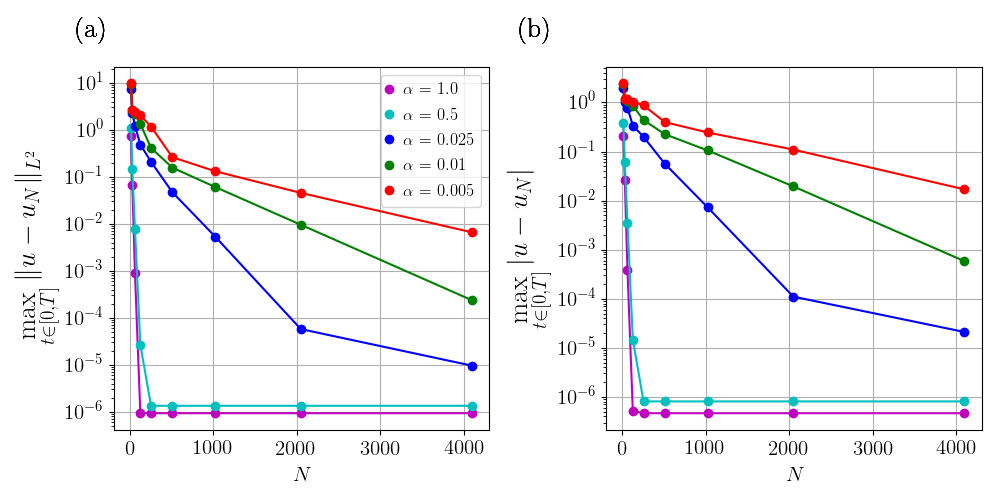
\includegraphics[width=15cm]{Figures/Galerkin/Graphics/alphas_Error_N.png}
		\caption{(a) $L^2$-norm between the exact solution and its approximations using Galerkin method. (b) Max norm between the exact solution and its approximations.}
		\label{Galerkin_alphas}
	\end{figure}

	\newpage	
	\begin{figure}[H]
		\centering
		\caption{Numerical solution for (\ref{burgers}) using (\ref{full_discrete}) with $\alpha = 1.0$, $N=2048$, and $\Delta t = 1.0 \times 10^{-5}$.}
		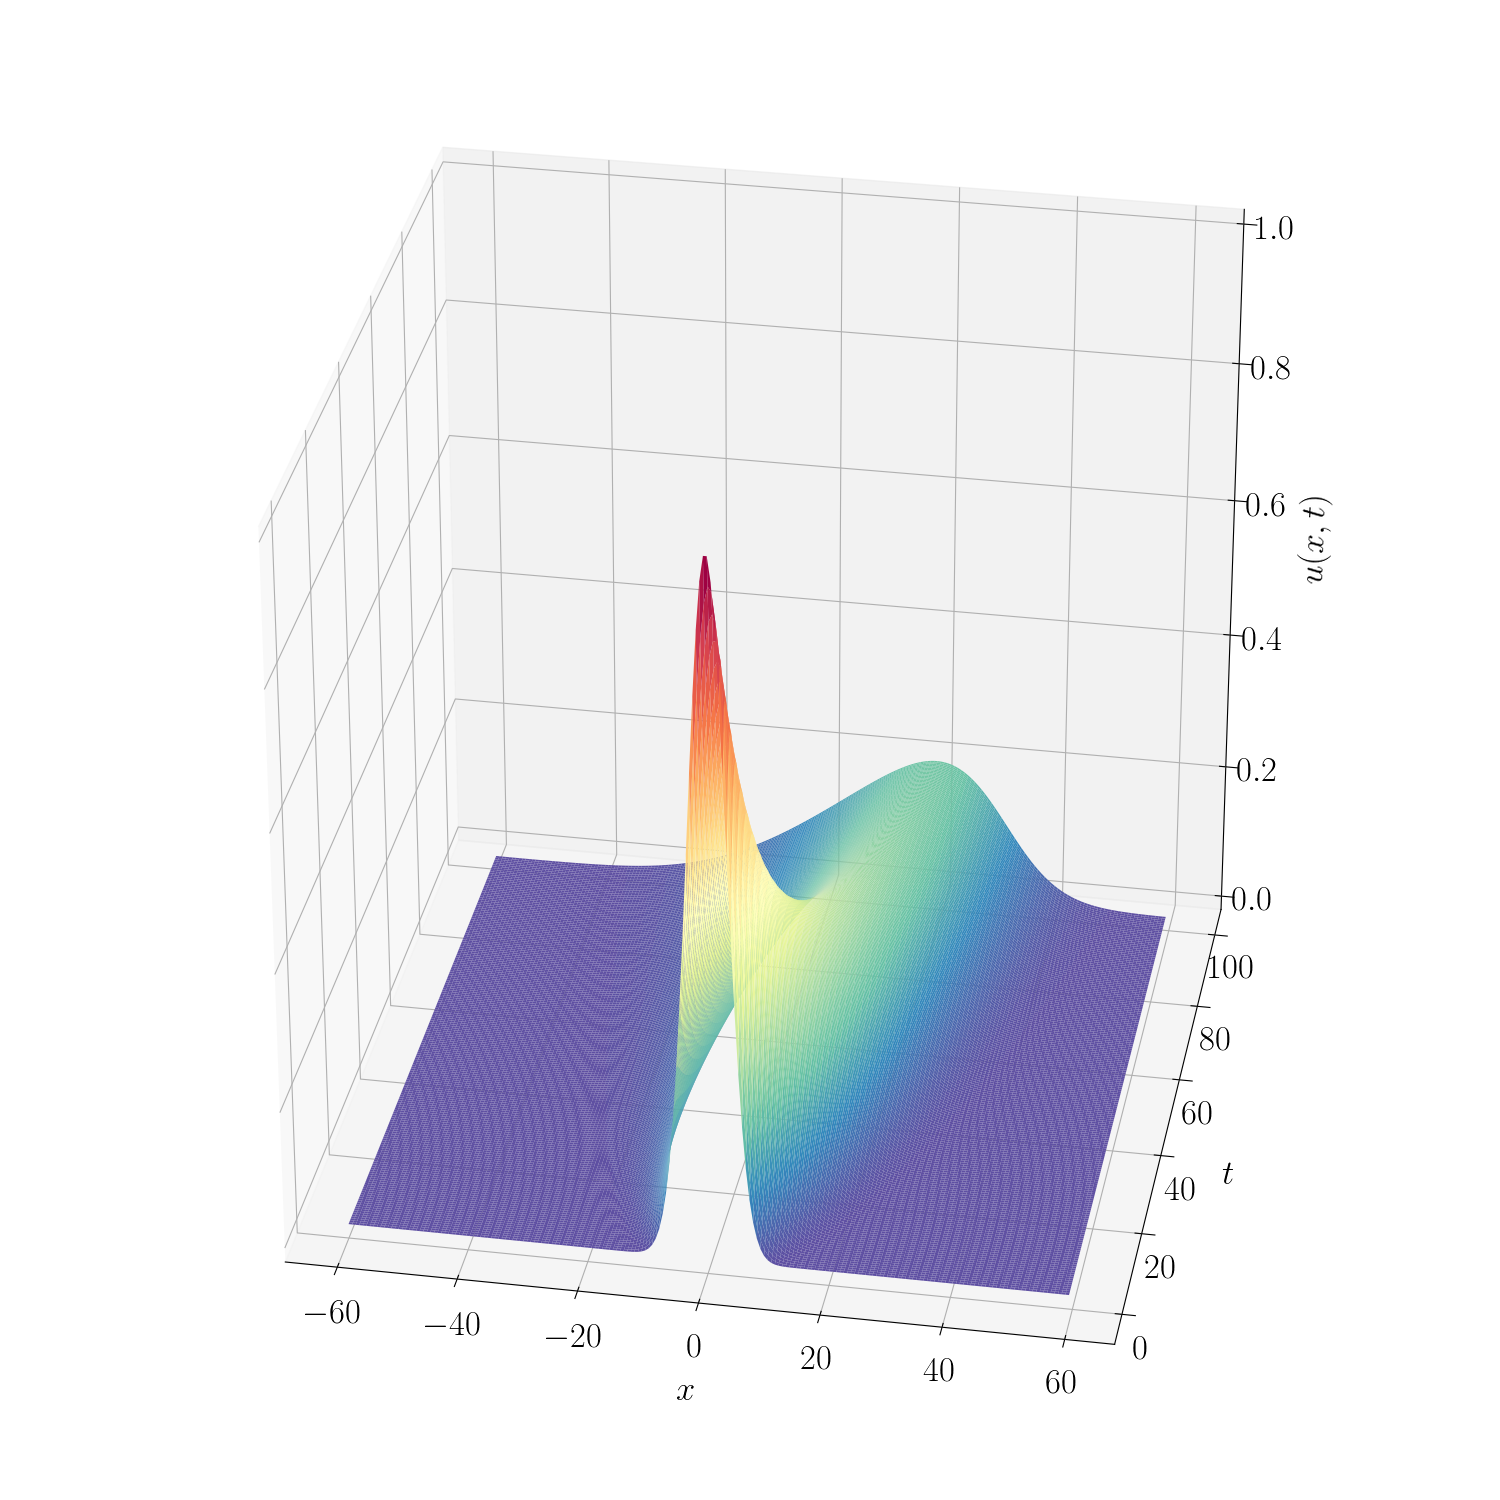
\includegraphics[width=12cm]{Figures/Galerkin/Graphics/eps=1.0/Numerical_Solution_alpha=1.png}
		\label{Galerkin_alpha=1}
		\caption{Numerical solution for (\ref{burgers}) using (\ref{full_discrete}) at the time $T = 100$ with $\alpha = 1.0$, and $\Delta t = 1.0 \times 10^{-5}$. (b) Point-wise error of approximation}
		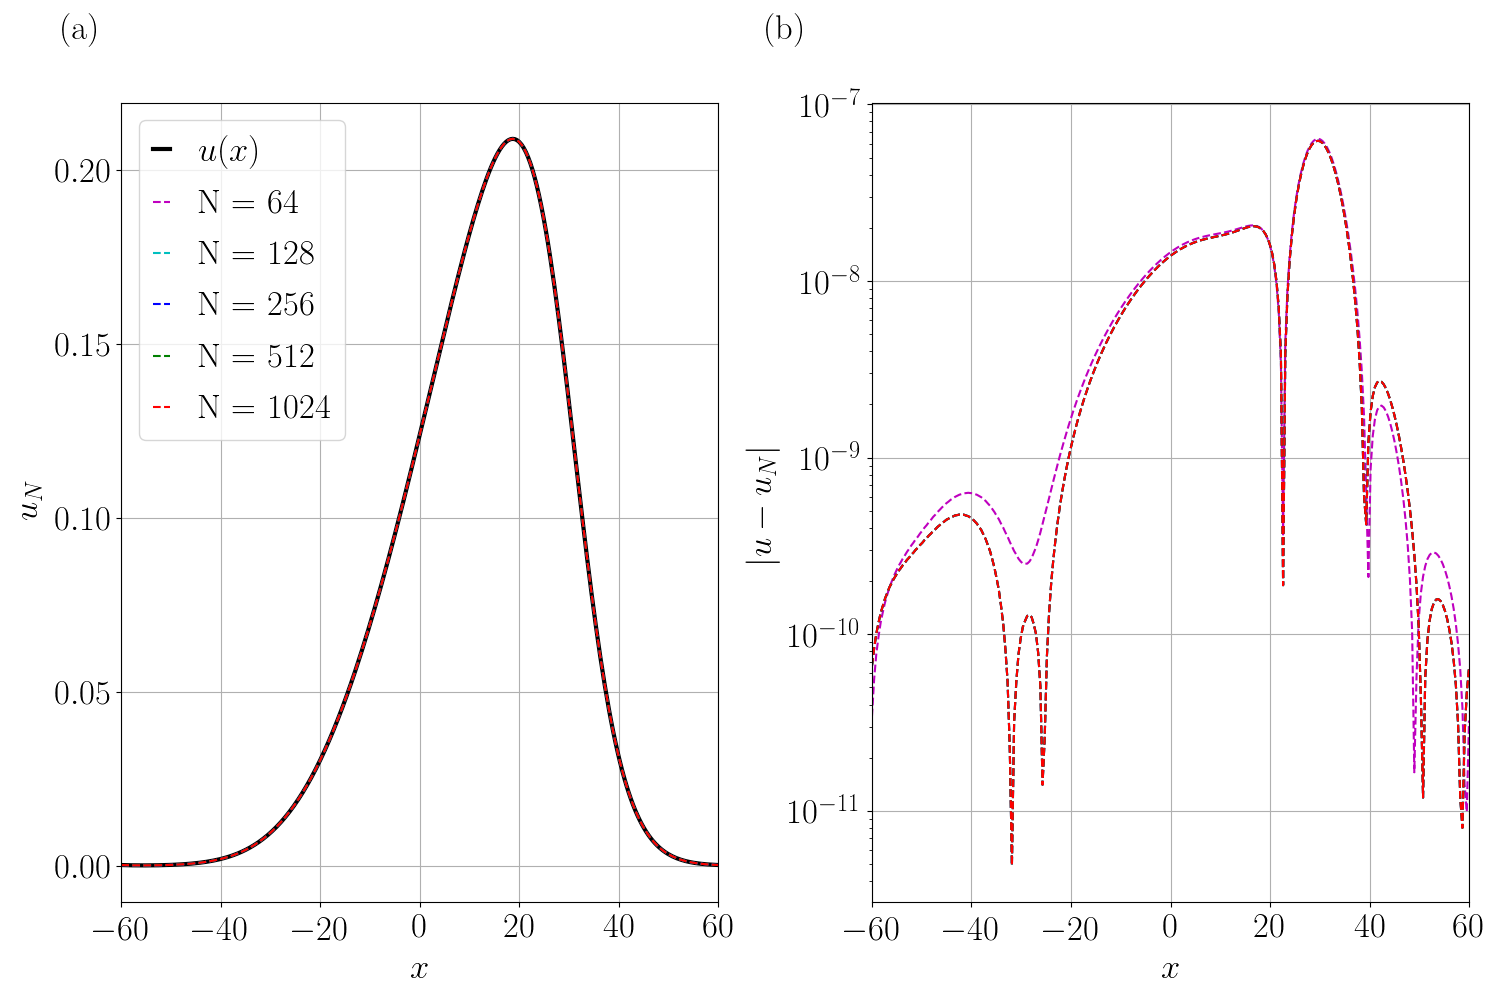
\includegraphics[width=12.5cm]{Figures/Galerkin/Graphics/eps=1.0/Numerical_Solution_alpha=1_T=100.png}
		\label{Galerkin_alpha=1_T}
	\end{figure}
	\begin{table}[H]
		\begin{tabular}{lcccc}
			\toprule
			\multicolumn{1}{c}{\textbf{Approximation}} & \multicolumn{4}{c}{\textbf{Error}} \\
			$\hspace{9mm}N$ & $\Delta t=1\times 10^{-2}$ & $\Delta t=1\times 10^{-3}$ & $\Delta t=1\times 10^{-4}$ & $\Delta t=1\times 10^{-5}$ \\
			\midrule
			\hspace{7mm} 16 & 0.72504    & 0.72504    & 0.72504    & 0.72504    \\
			\midrule
			\hspace{7mm} 32 & 6.90249 $\times 10 ^{-2}$   & 6.88052 $\times 10 ^{-2}$   & 6.87838 $\times 10 ^{-2}$   & 6.87816 $\times 10 ^{-2}$   \\
			\midrule
			\hspace{7mm} 64 & 1.23827 $\times 10 ^{-3}$  & 8.85367 $\times 10 ^{-4}$ & 8.80521 $\times 10 ^{-4}$ & 8.80410 $\times 10 ^{-4}$  \\
			\midrule
			\hspace{7mm} 128 & 9.43454 $\times 10 ^{-4}$ & 9.41793 $\times 10 ^{-5}$ & 9.41148 $\times 10 ^{-6}$ & 9.41827 $\times 10 ^{-7}$  \\
			\midrule
			\hspace{7mm} 256 & 9.43454 $\times 10 ^{-4}$ & 9.41793 $\times 10 ^{-5}$ & 9.41109 $\times 10 ^{-6}$ & 9.36411 $\times 10 ^{-7}$ \\
			\midrule
			\hspace{7mm} 512 & 9.43454 $\times 10 ^{-4}$ & 9.41793 $\times 10 ^{-5}$ & 9.41109 $\times 10 ^{-6}$ & 9.36411 $\times 10 ^{-7}$ \\
			\midrule
			\hspace{7mm} 1024 & $\ast$ & 9.41793 $\times 10^{-5}$ & 9.41109 $\times 10^{-6}$ & 9.36411 $\times 10^{-7}$              \\
			\midrule
			\hspace{7mm} 2048 & $\ast$ & $\ast$ & 9.41109 $\times 10^{-6}$ & 9.36411 $\times 10^{-7}$   \\
			\\
			\bottomrule
		\end{tabular}
		\caption{Error using $L^2$-norm with $\alpha = 1.0$}
		\label{Galerkin_tabla_L2_alpha=1}
		\vspace{1cm}
		\begin{tabular}{lcccc}
			\toprule
			\multicolumn{1}{c}{\textbf{Approximation Max}} & \multicolumn{4}{c}{\textbf{Error}} \\
			$\hspace{9mm}N$ & $\Delta t=1\times 10^{-2}$ & $\Delta t=1\times 10^{-3}$ & $\Delta t=1\times 10^{-4}$ & $\Delta t=1\times 10^{-5}$ \\
			\midrule
			\hspace{7mm} 16 & 0.203363    & 0.203333    & 0.203331    & 0.20333     \\
			\midrule
			\hspace{7mm} 32 & 2.64192 $\times 10 ^{-2}$   & 2.6248 $\times 10 ^{-2}$    & 2.62491 $\times 10 ^{-2}$  & 2.62492 $\times 10 ^{-2}$   \\
			\midrule
			\hspace{7mm} 64 & 6.93001 $\times 10 ^{-4}$ & 4.11641 $\times 10 ^{-4}$ & 3.85563 $\times 10 ^{-4}$ & 3.82972 $\times 10 ^{-4}$ \\
			\midrule
			\hspace{7mm} 128 & 4.74934 $\times 10 ^{-4}$ & 4.73649 $\times 10 ^{-5}$ & 4.74295 $\times 10 ^{-6}$ & 5.16105 $\times 10 ^{-7}$ \\
			\midrule
			\hspace{7mm} 256 & 4.74936 $\times 10 ^{-4}$ & 4.7368 $\times 10 ^{-5}$  & 4.72569 $\times 10 ^{-6}$ & 4.64922 $\times 10 ^{-7}$ \\
			\midrule
			\hspace{7mm} 512 & 4.74936 $\times 10 ^{-4}$ & 4.7368 $\times 10 ^{-5}$  & 4.72569 $\times 10 ^{-6}$ & 4.64922 $\times 10 ^{-4}$ \\
			\midrule
			\hspace{7mm} 1024 & * & 4.7368 $\times 10 ^{-5}$  & 4.72569 $\times 10 ^{-6}$ & 4.64922 $\times 10 ^{-7}$ \\
			\midrule
			\hspace{7mm} 2048 & * & * & 4.72569 $\times 10 ^{-6}$ & 4.64922 $\times 10 ^{-7}$ \\
			\\
			\bottomrule
		\end{tabular}
		\caption{Error using Max norm with $\alpha = 1.0$}
		\label{Galerkin_tabla_max_alpha=1}
	\end{table}

	\begin{figure}[H]
		\centering
		\caption{Numerical solution for (\ref{burgers}) using (\ref{full_discrete}) with $\alpha = 0.005$, $N=2048$, and $\Delta t = 1.0 \times 10^{-5}$.}
		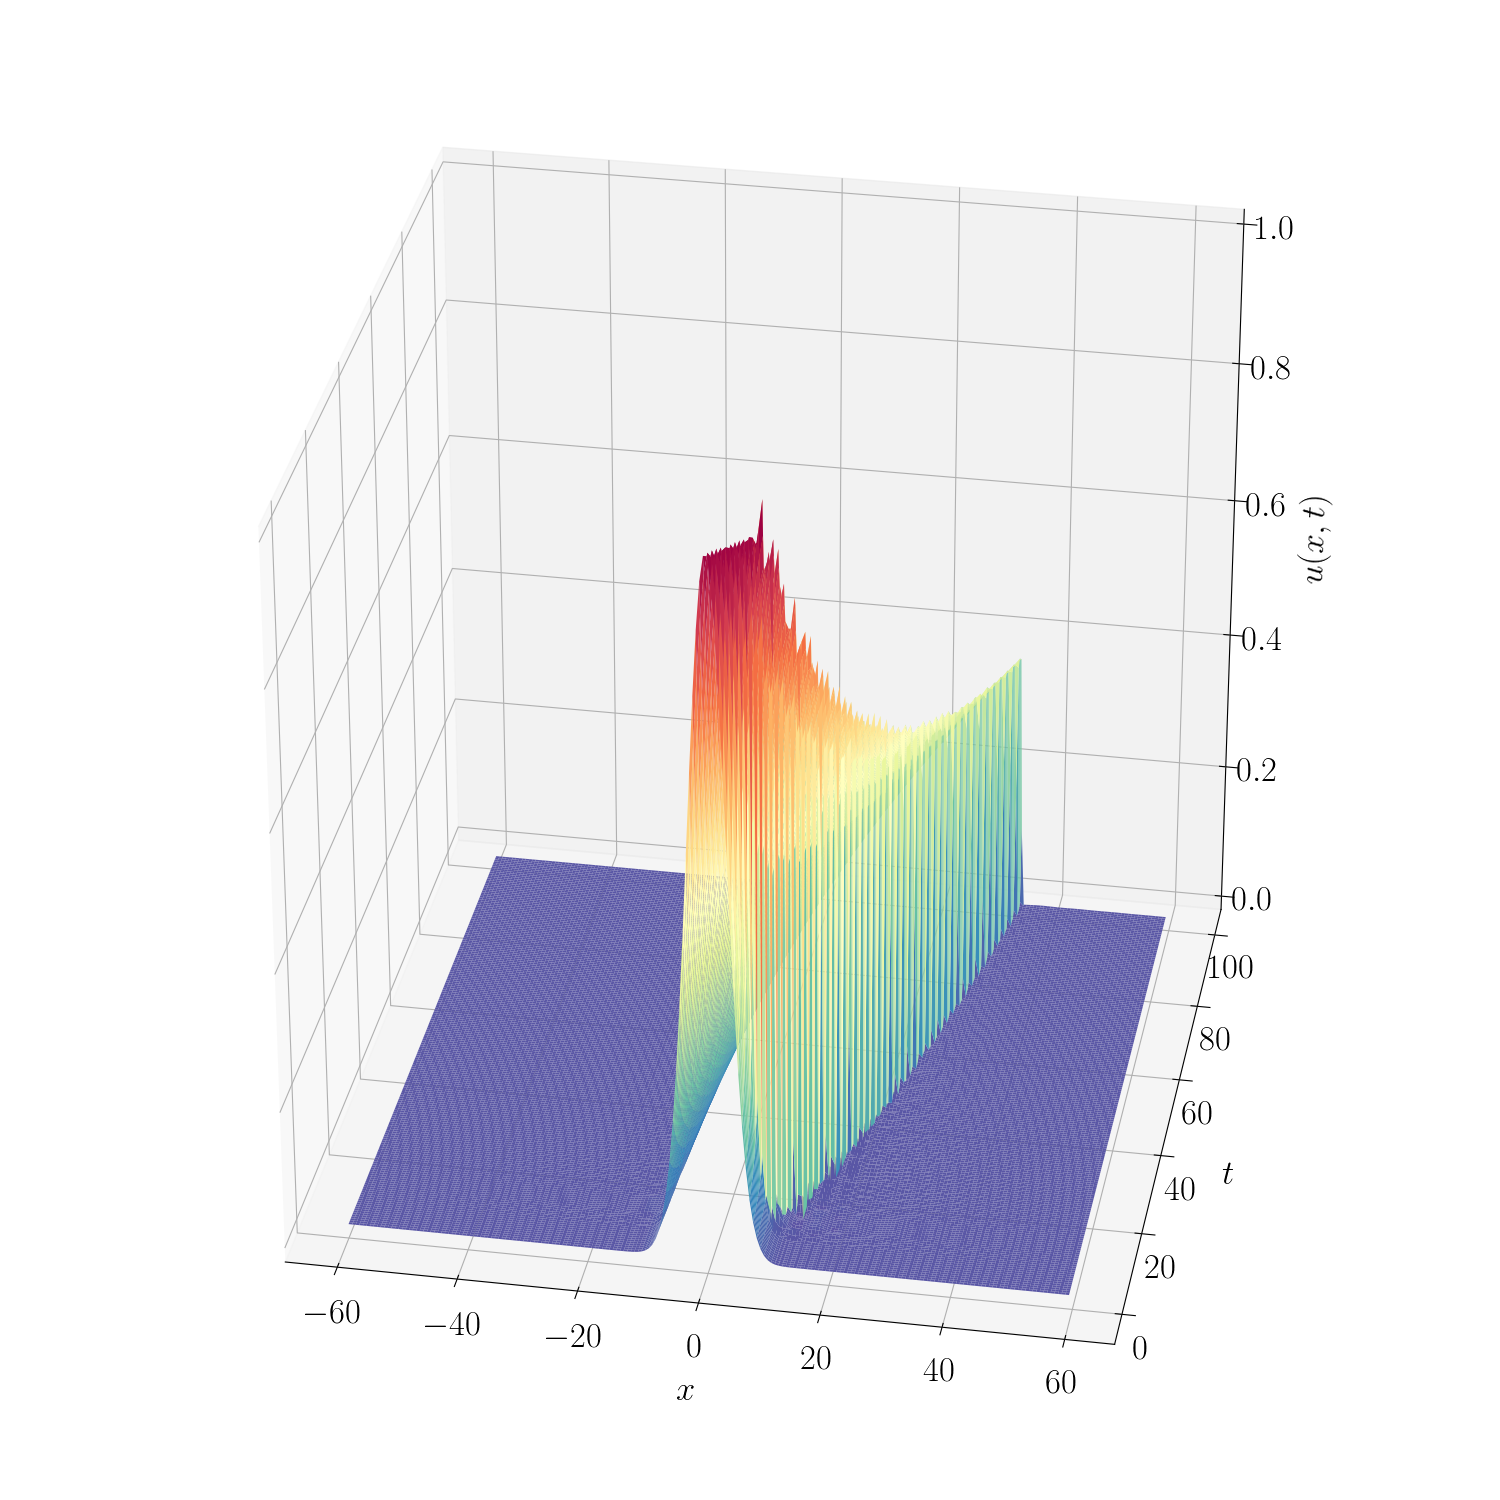
\includegraphics[width=12cm]{Figures/Galerkin/Graphics/eps=0.005/Numerical_Solution_alpha=0005.png}
		\caption{Numerical solution for (\ref{burgers}) using (\ref{full_discrete}) at the time $T = 100$ with $\alpha = 1.0$, and $\Delta t = 1.0 \times 10^{-5}$. (b) Point-wise error of approximation}
		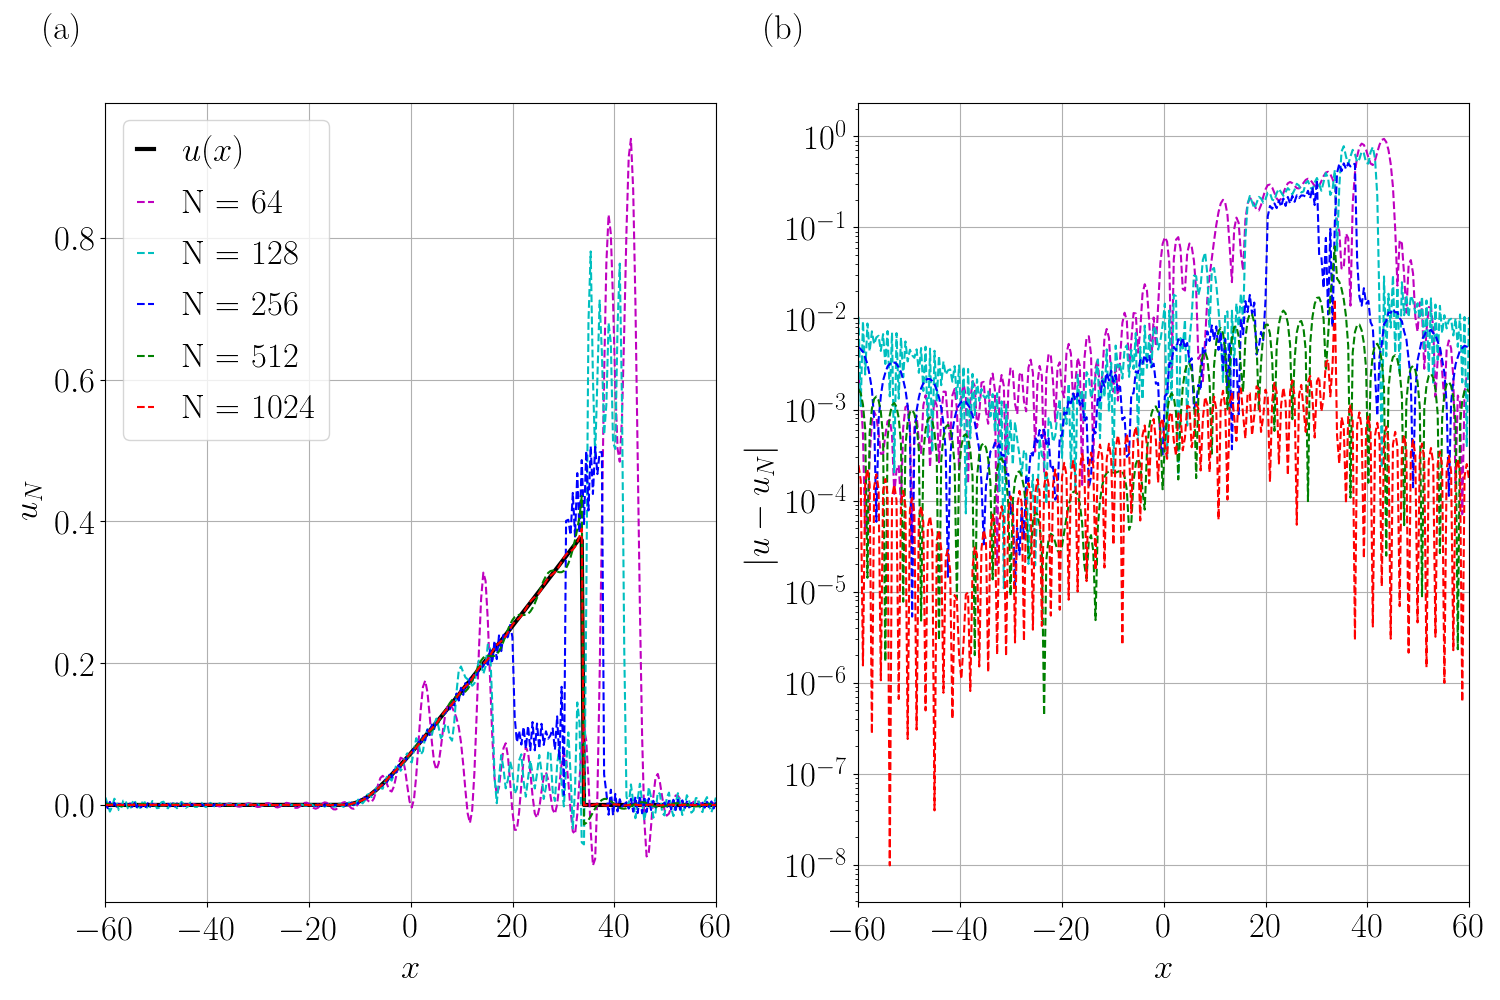
\includegraphics[width=12.5cm]{Figures/Galerkin/Graphics/eps=0.005/Numerical_Solution_alpha=0005_T=100.png}
		\label{Galerkin_alpha=005_T}
	\end{figure}
	
	\begin{table}[H]
	\begin{tabular}{lcccc}
		\toprule
		\multicolumn{1}{c}{\textbf{Approximation}} & \multicolumn{4}{c}{\textbf{Error}} \\
		$\hspace{9mm}N$ & $\Delta t=1\times 10^{-2}$ & $\Delta t=1\times 10^{-3}$ & $\Delta t=1\times 10^{-4}$ & $\Delta t=1\times 10^{-5}$ \\
		\midrule
		\hspace{7mm} 16 & 9.95328   & 9.91901    & 9.91597    & 9.91567    \\
		\midrule
		\hspace{7mm} 32 & 2.72607   & 2.70558    & 2.70347    & 2.70326    \\
		\midrule
		\hspace{7mm} 64 & 2.50343   & 2.45988    & 2.45543    & 2.45497    \\
		\midrule
		\hspace{7mm} 128 & 2.16142   & 2.06992    & 2.05918    & 2.05795    \\
		\midrule
		\hspace{7mm} 256 & 1.3658    & 1.19385    & 1.17602    & 1.17412    \\
		\midrule
		\hspace{7mm} 512 & 0.339826  & 0.265843   & 0.262164   & 0.261805   \\
		\midrule
		\hspace{7mm} 1024 & 0.161405  & 0.133743   & 0.131882   & 0.131699   \\
		\midrule
		\hspace{7mm} 2048 & 6.50292 $\times 10^{-2}$ & 4.70602 $\times 10^{-2}$ & 4.57371 $\times 10^{-2}$  & 4.56090 $\times 10^{-2}$  \\
		\midrule
		\hspace{7mm} 4096 & * & 7.26917 $\times 10^{-3}$ & 6.64157 $\times 10^{-3}$ & 6.60753 $\times 10^{-3}$ \\
		\\
		\bottomrule
	\end{tabular}
	\caption{Error using $L^2$-norm with $\alpha = 0.005$}
	\label{Galerkin_tabla_L2_alpha=005}
	\vspace{1cm}
	\begin{tabular}{lcccc}
		\toprule
		\multicolumn{1}{c}{\textbf{Approximation Max}} & \multicolumn{4}{c}{\textbf{Error}} \\
		$\hspace{9mm}N$ & $\Delta t=1\times 10^{-2}$ & $\Delta t=1\times 10^{-3}$ & $\Delta t=1\times 10^{-4}$ & $\Delta t=1\times 10^{-5}$ \\
		\midrule
		\hspace{7mm} 16 & 2.50002  & 2.48992   & 2.48891   & 2.48881   \\
		\midrule
		\hspace{7mm} 32 & 1.21263  & 1.20544   & 1.2047    & 1.20463   \\
		\midrule
		\hspace{7mm} 64 & 1.21269  & 1.17736   & 1.17517   & 1.17495   \\
		\midrule
		\hspace{7mm} 128 & 1.10164  & 1.03493   & 1.03093   & 1.03048   \\
		\midrule
		\hspace{7mm} 256 & 0.954369 & 0.881472  & 0.873392  & 0.87259   \\
		\midrule
		\hspace{7mm} 512 & 0.665071 & 0.418735  & 0.398664  & 0.396931  \\
		\midrule
		\hspace{7mm} 1024 & 0.241841 & 0.244188  & 0.244437  & 0.244461  \\
		\midrule
		\hspace{7mm} 2048 & 0.133067 & 0.104675  & 0.109151  & 0.109596  \\
		\midrule
		\hspace{7mm} 4096 & * & 2.37273  $\times 10 ^{-2}$ & 1.75687  $\times 10 ^{-2}$ & 1.69531  $\times 10 ^{-2}$\\
		\\
		\bottomrule
	\end{tabular}
	\caption{Error using Max norm with $\alpha =0.005$}
	\label{Galerkin_tabla_max_alpha=005}
	\end{table}
	
	\newpage
	\subsection{Collocation Simulations}
	As before, we require the residual to be zero, but now only at points $ x_j $, i.e.,
	\begin{align*}
		R_{N} (x_j, t) = \frac{\partial u_N}{\partial t} (x_j, t) - \frac{\partial^2 u_N }{\partial x^2} (x_j, t) + \frac{1}{2} \mathcal{J}_N \left(u^2_N \right)_x (x_j, t) - f(x_j, t) = 0
	\end{align*}
	
	The above defines $N$ ordinary differential equations for $u_N (x_j , t)$ with initial conditions $u_N (x_j, 0) = u_0(x_j)$, but firstly, we need to define again the linear transformation from $I_0 = [0, 2 \pi]$ to $I = [a, b]$ given by $T (z) = P z + a$, where $P = \frac {b - a}{2 \pi}$ and $z \in I_0$ is a scale factor. \\
	
	If Setting as follows
	\begin{align*}
		u_N (t) &= (u_N (x_0 , t), u_N (x_1 , t), \dots , u_N (x_{N} , t))^T, \\
		f_N(t) &= (f(x_0 , t), f(x_1 , t), \dots , f(x_{N} , t))^T,
	\end{align*} 
	
	the above system of ordinary differential equations can be written as follows
	\begin{align*}
		\frac{d u_N (t)}{dt} + \frac{1}{2} D_N u^2_N (t) - D_N^2 u_N (t) - f_N (t) = 0,
	\end{align*}
	
	where $D_N$ is the matrix given by (\ref{matrix_DN_odd}) already scaled by factor $P$, that represents discrete Fourier differentiation. \\
	
	Solving the above equation using backward Euler for nonlinear term gives us
	\begin{align}
		u_N (t_{i + 1} ) = u_N (t_i) + \Delta t \left[ D_N^2 u_N (t_i) - \frac{1}{2} D_N u^2_N (t_{i+1}) + f_N (t_i) \right].
	\end{align}
	
	For the following numerical simulations that we will describe, we will use the discretization of the problem already described, which was the following
	\begin{align}
		\label{Collocation_full_discrete}
		u_N (t_{i + 1} ) = u_N (t_i) + \Delta t \left[p^2 D_N^2 u_N (t_i) - \frac{1}{2} p D_N u^2_N (t_{i+1}) \right].
	\end{align}
	
	The discretization of the time variable $t$ over the interval $[0, T]$ is given by
	\begin{align*}
		t_i = i \Delta t, \hspace{2mm} i = 0, 1, \dots, T,
	\end{align*} 
	
	and for the spatial variable $x$ over the interval $[x_L, x_R]$ is given by $x_j = p z_n + x_L$, where $p = \frac{x_R - x_L}{2 \pi}$, and  
	\begin{align*}
		z_j = \frac{2 \pi j}{2N + 1}, \hspace{2mm} j = 0, 1, \dots, N.
	\end{align*}
	
	Finally to evaluate the numerical solution the following expression will be used
	\begin{align*}
		u_N(x, t_j) = \displaystyle \sum_{|n| \leq N} \hat{u}_j (t_i) e^{inx}
	\end{align*}
	
	For the numerical study, we will use the analytical solution of (\ref {burgers}) given by (\ref{exact_sol}), establishing the following initial condition
	\begin{align}
		u_0 (x) = e^{0.05 x^2}, \hspace{3mm} x \in [x_L, x_R] 
	\end{align}
	
	In the figure \ref{Collocation_alphas} shows the maximum distance over every $t \in [0, 100]$ between the exact solution and its approximations given by (\ref{Collocation_full_discrete}) for $N = 2^m$, $m = 4, \dots, 12$, $\Delta t = 1.0 \times 10^{-5}$, and different values of $\alpha$. Furthermore, in Tables \ref{Collocation_tabla_L2_alpha=1} and \ref{Collocation_tabla_max_alpha=1}, we can see the numerical values ​​of these distances for different configurations of $N$ and $\Delta t$. Similarly, in Tables \ref{Collocation_tabla_L2_alpha=005} and \ref{Collocation_tabla_max_alpha=005} but for $\alpha = 0.005$.
	
	\begin{figure}[H]
		\centering
		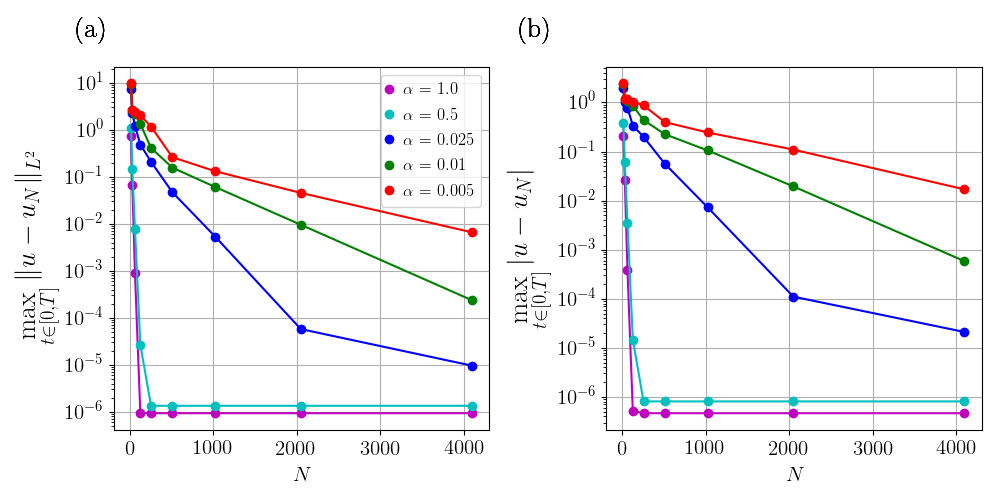
\includegraphics[width=12cm]{Figures/Galerkin/Graphics/alphas_Error_N.png}
		\caption{(a) $L^2$-norm between the exact solution and its approximations using Collocation method. (b) Max norm between the exact solution and its approximations.}
		\label{Collocation_alphas}
	\end{figure}

	\newpage
	\begin{figure}[H]
		\centering
		\caption{Numerical solution for (\ref{burgers}) using (\ref{Collocation_full_discrete}) with $\alpha = 1.0$, $N=2048$, and $\Delta t = 1.0 \times 10^{-5}$.}
		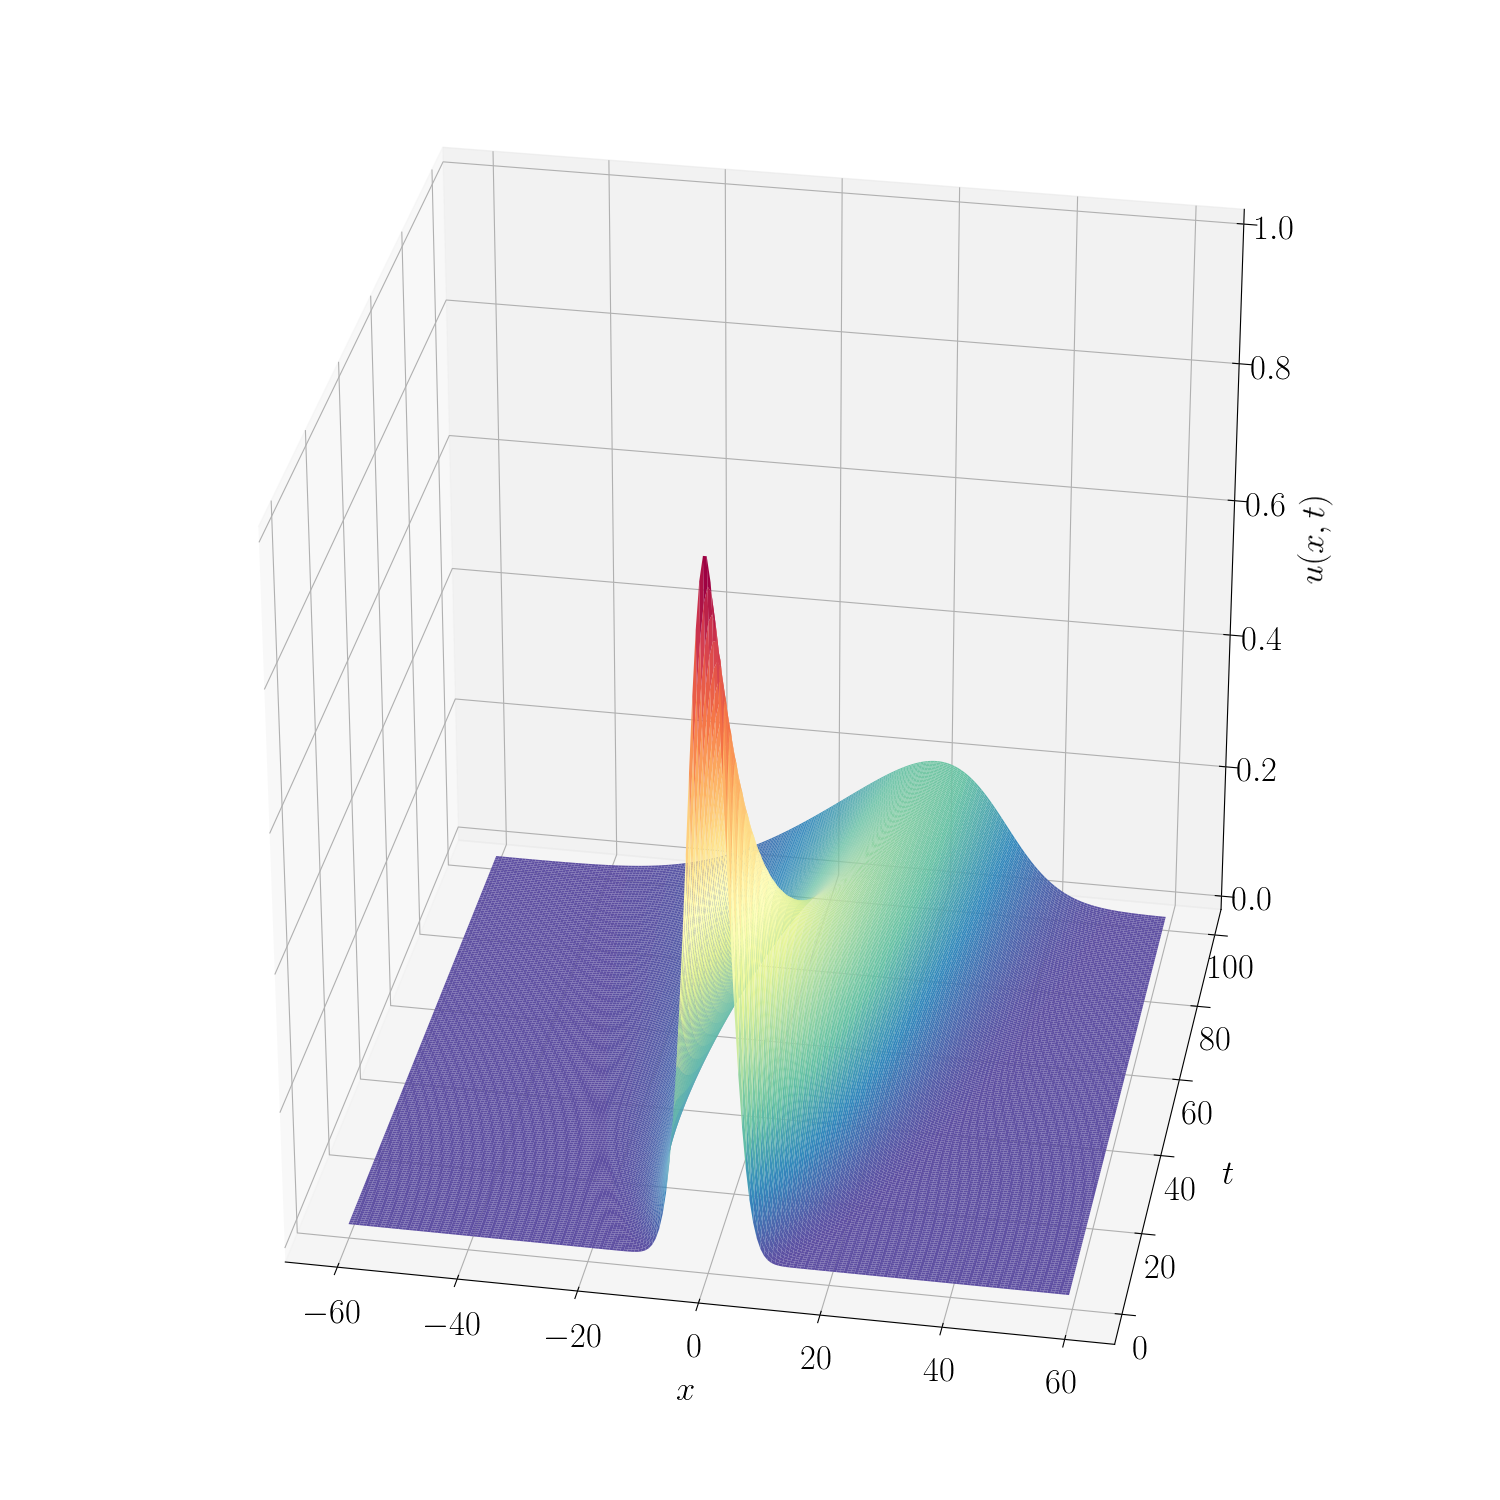
\includegraphics[width=12cm]{Figures/Collocation/Graphics/eps=1.0/Numerical_Solution_alpha=1.png}
		\label{Collocation_alpha=1}
		\caption{Numerical solution for (\ref{burgers}) using (\ref{Collocation_full_discrete}) at the time $T = 100$ with $\alpha = 1.0$, and $\Delta t = 1.0 \times 10^{-5}$. (b) Point-wise error of approximation}
		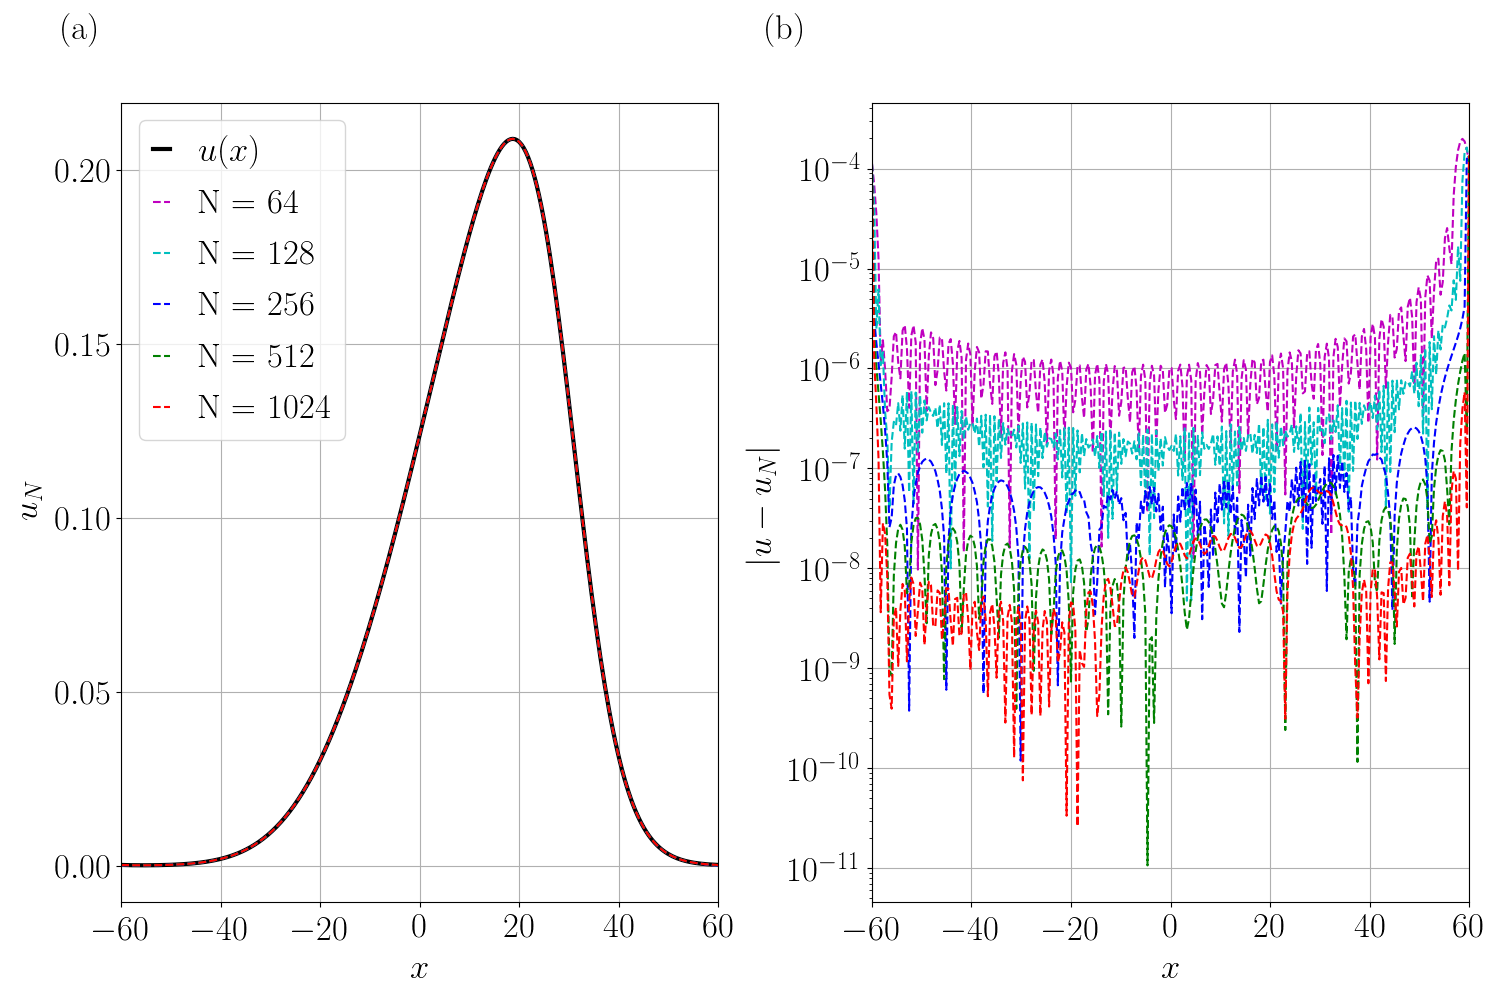
\includegraphics[width=12.5cm]{Figures/Collocation/Graphics/eps=1.0/Numerical_Solution_alpha=1_T=100.png}
		\label{Collocation_alpha=1_T}
	\end{figure}
	\begin{table}[H]
		\begin{tabular}{lcccc}
			\toprule
			\multicolumn{1}{c}{\textbf{Approximation}} & \multicolumn{4}{c}{\textbf{Error}} \\
			$\hspace{9mm}N$ & $\Delta t=1\times 10^{-2}$ & $\Delta t=1\times 10^{-3}$ & $\Delta t=1\times 10^{-4}$ & $\Delta t=1\times 10^{-5}$ \\
			\midrule
			\hspace{7mm} 16 & 0.721112    & 0.721112    & 0.721112    & 0.721112    \\
			\midrule
			\hspace{7mm} 32 & 4.71797 $\times 10^{-2}$   & 4.72892 $\times 10^{-2}$   & 4.73004 $\times 10^{-2}$   & 4.73015 $\times 10^{-2}$   \\
			\midrule
			\hspace{7mm} 64 & 1.17954 $\times 10^{-3}$  & 7.35344 $\times 10^{-4}$ & 7.27561 $\times 10^{-4}$ & 7.27283 $\times 10^{-4}$  \\
			\midrule
			\hspace{7mm} 128 & 9.43454 $\times 10^{-4}$ & 1.75152 $\times 10^{-4}$ & 1.74583 $\times 10^{-4}$ & 1.74574 $\times 10^{-4}$ \\
			\midrule
			\hspace{7mm} 256 & 9.43454 $\times 10^{-4}$ & 1.15509 $\times 10^{-4}$ & 1.14669 $\times 10^{-4}$ & 1.14659 $\times 10^{-4}$ \\
			\midrule
			\hspace{7mm} 512 & 9.43454 $\times 10^{-4}$ & 9.41793 $\times 10^{-5}$ & 7.78847 $\times 10^{-5}$ & 7.78707 $\times 10^{-5}$ \\
			\midrule
			\hspace{7mm} 1024 & 0           & 9.41793 $\times 10^{-5}$ & 5.32213 $\times 10^{-5}$ & 5.32019 $\times 10^{-5}$ \\
			\midrule
			\hspace{7mm} 2048 & 0           & 0           & 3.56779 $\times 10^{-5}$ & 3.56498 $\times 10^{-5}$ \\
			\midrule
			\hspace{7mm} 4096 & 0           & 0           & 2.24122 $\times 10^{-5}$ & 0           \\
			\\
			\bottomrule
		\end{tabular}
		\caption{Error using $L^2$-norm with $\alpha=1.0$}
		\label{Collocation_tabla_L2_alpha=1}
		\vspace{1cm}
		\begin{tabular}{lcccc}
			\toprule
			\multicolumn{1}{c}{\textbf{Approximation Max}} & \multicolumn{4}{c}{\textbf{Error}} \\
			$\hspace{9mm}N$ & $\Delta t=1\times 10^{-2}$ & $\Delta t=1\times 10^{-3}$ & $\Delta t=1\times 10^{-4}$ & $\Delta t=1\times 10^{-5}$ \\
			\midrule
			\hspace{7mm} 16 & 0.317617    & 0.317617    & 0.317617    & 0.317617    \\
			\midrule
			\hspace{7mm} 32 & 1.95279 $\times 10 ^{-2}$  & 1.96812 $\times 10 ^{-2}$   & 1.96965 $\times 10 ^{-2}$   & 1.96981 $\times 10 ^{-2}$   \\
			\midrule
			\hspace{7mm} 64 & 6.21793 $\times 10 ^{-4}$ & 2.9813 $\times 10 ^{-4}$  & 2.80086 $\times 10 ^{-4}$ & 2.78934 $\times 10 ^{-4}$ \\
			\midrule
			\hspace{7mm} 128 & 4.74952 $\times 10 ^{-4}$ & 1.64746 $\times 10 ^{-4}$ & 1.6473 $\times 10 ^{-4}$  & 1.64728 $\times 10 ^{-4}$ \\
			\midrule
			\hspace{7mm} 256 & 4.74936 $\times 10 ^{-4}$ & 1.52482 $\times 10 ^{-4}$ & 1.52467 $\times 10 ^{-4}$ & 1.52465 $\times 10 ^{-4}$ \\
			\midrule
			\hspace{7mm} 512 & 4.74936 $\times 10 ^{-4}$ & 1.47249 $\times 10 ^{-4}$ & 1.47234 $\times 10 ^{-4}$ & 1.47232 $\times 10 ^{-4}$ \\
			\midrule
			\hspace{7mm} 1024 & 0           & 1.45032 $\times 10 ^{-4}$ & 1.45017 $\times 10 ^{-4}$ & 1.45016 $\times 10 ^{-4}$ \\
			\midrule
			\hspace{7mm} 2048 & 0           & 0           & 1.43941 $\times 10 ^{-4}$ & 1.4394 $\times 10 ^{-4}$ \\
			\midrule
			\hspace{7mm} 4096 & 0           & 0           & 1.43411 $\times 10 ^{-4}$ & 0           \\
			\\
			\bottomrule
		\end{tabular}
		\caption{Error using Max norm with $\alpha=1.0$}
		\label{Collocation_tabla_max_alpha=1}
	\end{table}
	
	
	\begin{figure}[H]
		\centering
		\caption{Numerical solution for (\ref{burgers}) using (\ref{Collocation_full_discrete}) with $\alpha = 0.005$, $N=2048$, and $\Delta t = 1.0 \times 10^{-5}$.}
		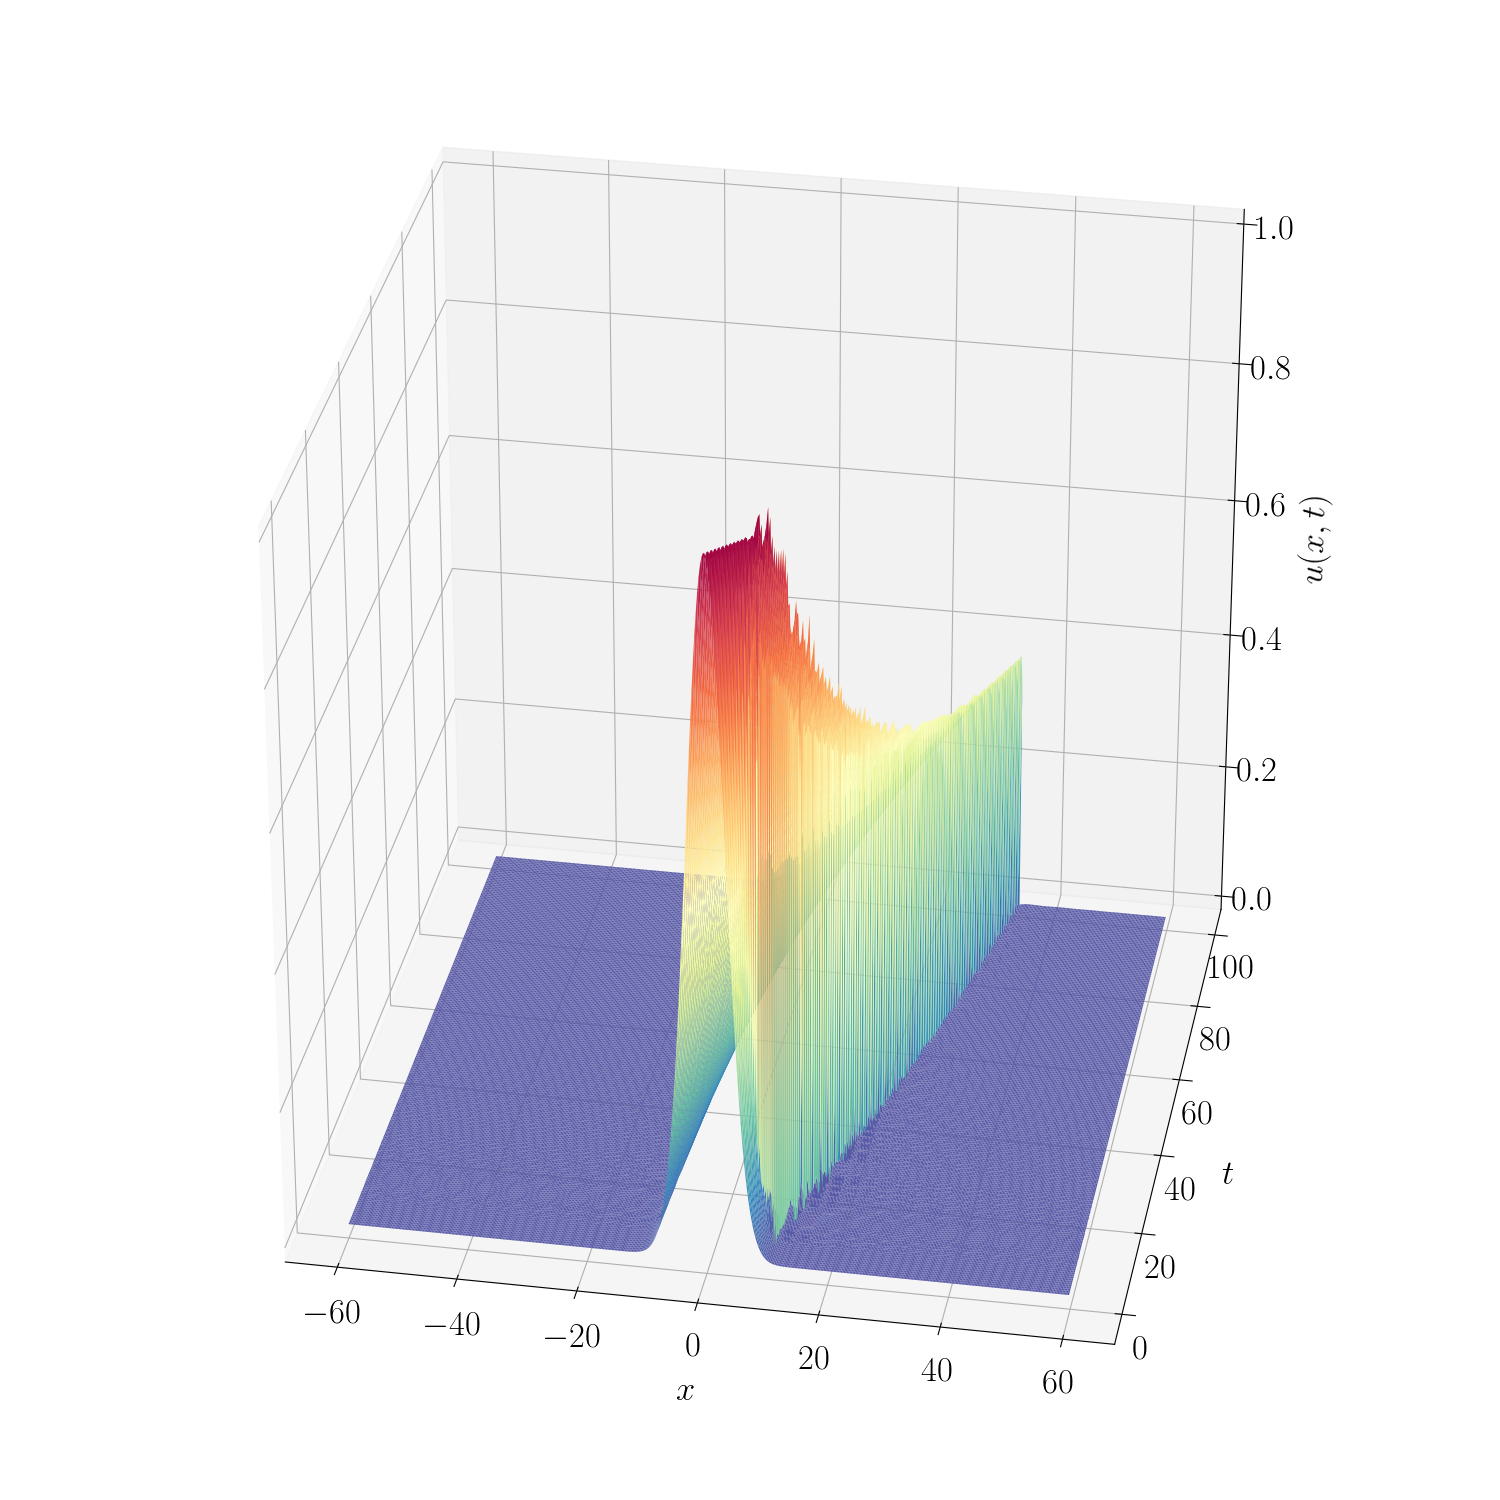
\includegraphics[width=12cm]{Figures/Collocation/Graphics/eps=0.005/Numerical_Solution_alpha=0005.png}
		\label{Collocation_alpha=005}
		\caption{Numerical solution for (\ref{burgers}) using (\ref{Collocation_full_discrete}) at the time $T = 100$ with $\alpha = 0.005$, and $\Delta t = 1.0 \times 10^{-5}$. (b) Point-wise error of approximation.}
		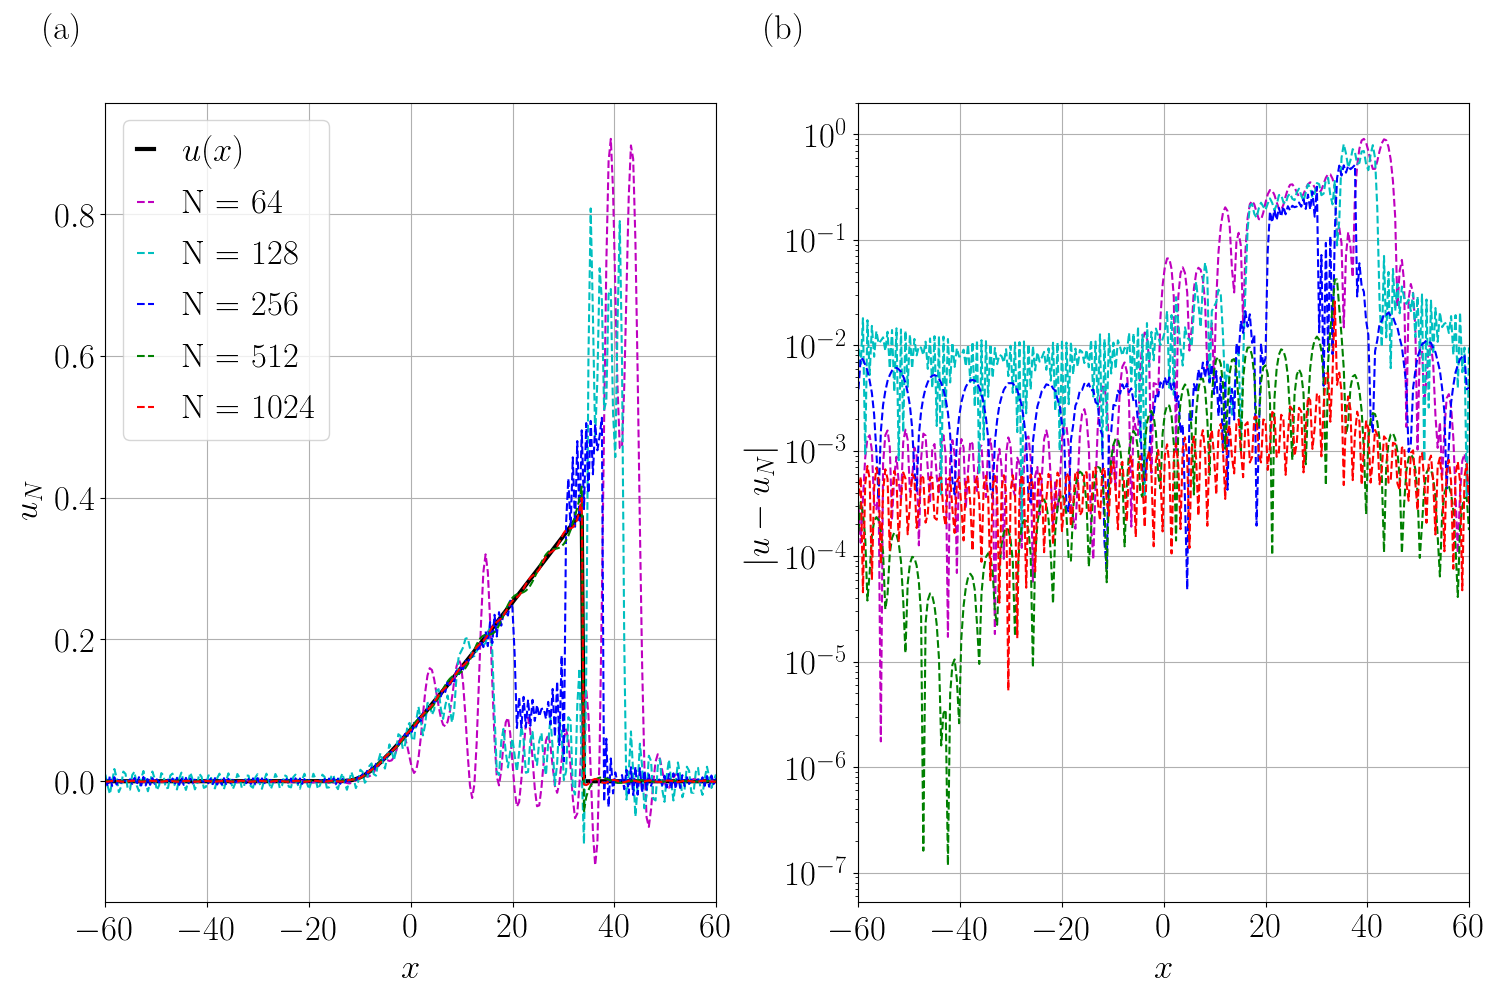
\includegraphics[width=12.5cm]{Figures/Collocation/Graphics/eps=0.005/Numerical_Solution_alpha=0005_T=100.png}
		\label{Collocation_alpha=005_T}
	\end{figure}
	%L2
	
	\begin{table}[H]
	\begin{tabular}{lcccc}
		\toprule
		\multicolumn{1}{c}{\textbf{Approximation}} & \multicolumn{4}{c}{\textbf{Error}} \\
		$\hspace{9mm}N$ & $\Delta t=1\times 10^{-2}$ & $\Delta t=1\times 10^{-3}$ & $\Delta t=1\times 10^{-4}$ & $\Delta t=1\times 10^{-5}$ \\
		\midrule
		\hspace{7mm} 16 & 1.36189   & 1.35883    & 1.35852   & 1.35849   \\
		\midrule
		\hspace{7mm} 32 & 2.67506   & 2.65305    & 2.65078   & 2.65055   \\
		\midrule
		\hspace{7mm} 64 & 2.50365   & 2.45855    & 2.45432   & 2.45387   \\
		\midrule
		\hspace{7mm} 128 & 2.15795   & 2.0632     & 2.05589   & 2.05497   \\
		\midrule
		\hspace{7mm} 256 & 1.362     & 1.18393    & 1.16697   & 1.16532   \\
		\midrule
		\hspace{7mm} 512 & 0.350775  & 0.304595   & 0.300865  & 0.300499  \\
		\midrule
		\hspace{7mm} 1024 & 0.168462  & 0.140332   & 0.13803   & 0.137804  \\
		\midrule
		\hspace{7mm} 2048 & 6.56161 $\times 10^{-2}$ & 4.63808 $\times 10^{-2}$  & 4.49226 $\times 10^{-2}$ & 4.47813 $\times 10^{-2}$ \\
		\midrule
		\hspace{7mm} 4096 & 0         & 7.66246 $\times 10^{-3}$ & 6.9909 $\times 10^{-3}$ & 0         \\
		\\
		\bottomrule
	\end{tabular}
	\caption{Error using $L^2$-norm with $\alpha=0.005$}
	\label{Collocation_tabla_L2_alpha=005}
	\vspace{1cm}
	\begin{tabular}{lcccc}
		\toprule
		\multicolumn{1}{c}{\textbf{Approximation Max}} & \multicolumn{4}{c}{\textbf{Error}} \\
		$\hspace{9mm}N$ & $\Delta t=1\times 10^{-2}$ & $\Delta t=1\times 10^{-3}$ & $\Delta t=1\times 10^{-4}$ & $\Delta t=1\times 10^{-5}$ \\
		\midrule
		\hspace{7mm} 16 & 0.695784 & 0.695659  & 0.695646  & 0.695645 \\
		\midrule
		\hspace{7mm} 32 & 1.20278  & 1.19418   & 1.19329   & 1.1932   \\
		\midrule
		\hspace{7mm} 64 & 1.22454  & 1.18903   & 1.18507   & 1.18467  \\
		\midrule
		\hspace{7mm} 128 & 1.11999  & 1.0238    & 1.01754   & 1.01701  \\
		\midrule
		\hspace{7mm} 256 & 0.927954 & 0.877058  & 0.872508  & 0.87201  \\
		\midrule
		\hspace{7mm} 512 & 0.664133 & 0.415288  & 0.39714   & 0.395563 \\
		\midrule
		\hspace{7mm} 1024 & 0.247742 & 0.259451  & 0.260605  & 0.26072  \\
		\midrule
		\hspace{7mm} 2048 & 0.126824 & 0.103297  & 0.107102  & 0.10748  \\
		\midrule
		\hspace{7mm} 4096 & 0        & 2.04624 $\times 10 ^{-2}$ & 1.76513  $\times 10 ^{-2}$ & 0        \\
		\\
		\bottomrule
	\end{tabular}
	\caption{Erro using Max norm with $\alpha=0.005$}
	\label{Collocation_tabla_max_alpha=005}
	\end{table}
	
	\newpage
	\subsection{Solutions for Small Viscosity Coefficients}
	Let $u \in H^1_p ([0,2 \pi])$ a periodic function such that is the solution of the following initial value problem
		\begin{align}
			\label{Inviscid}
			\left \lbrace \begin{array}{ll}
				\frac{\partial u(x, t)}{\partial t} = -u(x, t) \frac{\partial u(x, t)}{\partial x}, \\
				\\
				u(x, 0) = u_0(x), \hspace{2mm} x \in [0, 2 \pi].
			\end{array} \right .  
		\end{align}
		
		Notar que $u(x, t) \frac{\partial u(x, t)}{\partial x} = \frac{1}{2} \partial_x \left[ u(x, t) \right]^2$,
		y entonces procedemos a proyectar el problema anterior como antes para obtener
		\begin{align}
			\left \lbrace \begin{array}{ll}
				\frac{\partial \mathcal{P}_N u(x, t)}{\partial t} = - \frac{1}{2} \partial_x \left[ \mathcal{P}_N u(x, t) \right]^2, \\
				\\
				\mathcal{P}_N u(x, 0) = \mathcal{P}_N u_0(x), \hspace{2mm} x \in [0, 2 \pi].
			\end{array} \right .  
		\end{align}
		
		y haciendo el mismo procedimiento nos da
		\begin{align*}
			\left\langle \frac{\partial \mathcal{P}_N u(x, t)}{\partial t}, \phi_n  \right\rangle = & \left\langle\frac{in}{2} \left( \sum_{ |p| \leq N} \hat{u}_p (t) \phi_p \right) \left( \sum_{ |q| \leq N} \hat{u}_q (t) \phi_q \right), \phi_n \right\rangle \\
			=& - \frac{in}{2} \left\langle \sum_{ |p| \leq N} \sum_{ |q| \leq N} \hat{u}_p (t) \hat{u}_q (t) \phi_{p + q}, \phi_n \right \rangle \\
			=& - in \pi \sum_{ p + q = n} \hat{u}_p (t) \hat{u}_q (t), \hspace{2mm} |q|, |p| \leq N
		\end{align*}
		
		\noindent Asi, obtenemos el siguiente sistema acoplado de ecuaciones diferenciales no lineales
		\begin{align*}
			\frac{d \hat{u}_n (t)}{dt} = - \frac{in}{2}  \sum_{ p + q = n} \hat{u}_p (t) \hat{u}_q (t), \hspace{2mm} |q|, |p| \leq N 
		\end{align*}
		el cual ya no es posible obtener una solucion explicita con los metodos convencionales, e incluso implementar un metodo numerico para obtener una aproximacion es complicado.
		
		Sin embargo, el problema puede ser resuelto usando el operador interpolacion teniendo algo de ventaja. Recordar que al aplicar el operador $\mathcal{J}_N$ a la funcion $u$ es como sigue
		\begin{align*}
			\mathcal{J}_N u (x, t) =  \displaystyle \sum_{j=0}^{2N} u_{N} (x_j, t) g_j (x)
		\end{align*}
		where $g_j (x)$ satisfies $g_j(x_i) = \delta_{ij}$, and then we have that $\mathcal{J}_N u(x_j) = u(x_j)$ for every $j$.\\
		
		Entonces, definiendo el vector $U_N (t)$ como en (?) e utilizando la matriz de diferenciacion dada por (\ref{matrix_DN_even}), podemos escribir el problema (\ref{Convection_Well}) como
		\begin{align*}
			\frac{d u_N (t)}{dt} = - \frac{1}{2} D_N \left[ u_N (t) \circ u_N (t) \right]
		\end{align*}
		donde $\circ$ representa el producto puntual del $u_N (t)$. \\
		
		Aunque el sistema anterior tambien es compliado obtener una solucion explicita, aplicar un metodo numerico para aproximar la solucion es mucho mas facil. Sin embargo, escoger un metodo numerico eficiente no es sencillo, pero conociendo la naturelza del problema original puede ser util. \\ 
		
		Vamos a dar a conocer algunos aspectos de las soluciones del problema (\ref{Convection_Well}). Multiplying for $u$ and integration over the space
		\begin{align*}
			\frac{1}{2} \frac{d}{dt} \displaystyle \int_{0}^{2 \pi} u^2(x, t) dx = - \int_{0}^{2 \pi} u^2(x, t) \frac{\partial u(x, t)}{\partial x} dx = - \frac{1}{3} u^3(x, t) \Big|^{2 \pi}_{0} = 0.
		\end{align*}
		So we have to
		\begin{align*}
			\| u(x, t) \| = \| u(x, 0) \|,  
		\end{align*}
		and therefore the solution is bounded. \\
		
		The above means that the energy is conserved, often referred to as the Burgers' equation without viscosity, and is in some sense the simplest nonlinear conservation law  where $u$ is conserved with a flux density given by $f(u) = \frac{u^2}{2}$.\\
		
		As we will see, the equation is a model example of systems in which solutions can generate singularities in finite time. As we will see, it is in this case of non-avoidable discontinuities of the solution, also called shock. \\
		
		We define the next curves $x = x(t)$ that start from a point $x_0$, and satisfies the following equation:
		\begin{align}
			\label{Curves}	
			\left \lbrace \begin{array}{ll}
				x' (t) = u(x(t), t), \hspace{2mm} t > 0, \\
				\\
				x(0) = x_0.
			\end{array} \right .  
		\end{align}
		When the solution $u = u(x, t)$ is locally Lipschitz in the variable $x$ and, say, it continues in time $t$, for every $x_0 \in \mathbb{R}$ the previous equation admits a unique local solution that we will call characteristic curve. Differentiating $u(x(t), t)$ with respect to time $t$, and using the equation above along with the one in the Example \ref{Convection_Well}, we obtain the following
		\begin{align*}
			\frac{d}{dt} [u(x(t), t)] &= x' (t) u_x (x(t), t) + u_t (x(t), t) \\
			&= u(x(t), t) u_x (x(t), t) - u(x(t), t) u_x (x(t), t) = 0
		\end{align*}
		
		In effect, the value of the solution $u$ along a characteristic curve, that is, $u(x(t), t)$ is independent of the time $t$. Therefore, the solutions are constant along the characteristic curves, and we also have to
		\begin{align*}
			u(x(t), t) = u (x(0), 0) = u_0 (x_0)
		\end{align*}
		
		So the solution to the problem (\ref{Curves}) is given by
		\begin{align*}
			x(t) = x_0 + u_0 (x_0) t, \hspace{2mm} t > 0.
		\end{align*}
		
		We see therefore that the characteristic curves are actually straight, and also the solution $u(x, t)$ can be written as
		\begin{align*}
			u(x, t) = u_0(x_0), \hspace{2mm} x_0 = x - u_0(x_0) t
		\end{align*}
		
		Note the following. Let $x_0$, $x_1$ be start points such that $x_0 < x_1$, then for some $t$ we have to
		\begin{align*}
			x_0 + u_0(x_0) t = x_1 + u_0 (x_1) t,
		\end{align*}
		
		which tells us that two characteristic curves that start from $ x_0 $ and $ x_1 $ respectively, are cut at a point $ (x, t) $, where the time $ t $ is given by
		\begin{align*}
			t = \frac{x_1 - x_0}{u_0 (x_0) - u_0 (x_1)} = - \frac{1}{u'_0(c)},
		\end{align*}
		
		for some $c \in (x_0, x_1)$. Therefore, if $(x, t)$ is a point where two characteristic curves are cut that start from $x_0$ and $x_1$ respectively, at this point the solution cannot be continuous. This can be easily seen since the solution is constant along the characteristic curves, and then we would have to $u(x, t) = u_0(x_0) = u_0(x_1)$, which is impossible if $u_0(x_0) \neq u_0(x_1)$. \\
		
		Therefore, the time when the discontinuity or shock occurs is given by
		\begin{align}
			\label{shock_time}	
			Tc = \min_{x \in \mathbb{R}} \left[  \frac{-1}{u'_0 (x)} \right]
		\end{align}
	
	The evolution of the profile of this solution simulates in a simplified way that of a marine wave that approaches the coast. As it do it profile curls until it breaks. Once it has broken, it slides to the shore without further deformation. \\
	
	Perfect or ideal fluids, while constituting interesting mathematical models, are still unrealistic to the extent that each fluid has a certain degree of viscosity. Something similar occurs within the framework of the Burgers equation. The presence of a viscosity term introduces an additional regularization effect in the nonlinear equation. The important thing, in this case, is that this regularization effect is effective for all time $ t> 0 $ to avoid shocks. To observer this, recall by (\ref{exact_sol}) that the solution to problem (\ref{burgers}) is given by
	\begin{align}
		\label{Sol_alpha}	
		u(x, t) = - 2 \alpha \frac{[G_x(\cdot, t) * g_{\alpha}] (x)}{[G(\cdot, t) * g_{\alpha}] (x)},
	\end{align}
	
	where $G$ is known as the fundamental solution or Gauss kernel, and is given by 
	\begin{align*}
		G(x, t) = (4 \pi t)^{-1/2} \exp(- x^2 / 4t)
	\end{align*}
	and $g_{\alpha}$ defined by 
	\begin{align*}
		g_{\alpha} (x) = \displaystyle e^{- \int_{-\infty}^{x} \frac{u_0 (s)}{2 \alpha} ds}
	\end{align*}
	
	From the previous expression for the solution $u$ of the viscous Burgers' equation, we can observe that it is globally defined for all $\alpha > 0$, and it is also of class $C^{\infty} (\mathbb{R} \times (0, \infty))$ for all $\alpha > 0$.
	
	This means that the introduction of the term viscosity or diffusion into the Burgers' equation, however small $\alpha > 0$, makes the solutions regular. Recall that in the Burgers' equation, in the absence of viscosity, shocks occur for a finite time $Tc$ and the solution was no longer continuous. The regularizing effect of the viscosity term $\alpha > 0$ is thus evident. Simultaneously, the solutions become global in time. 
	
	From (\ref{Sol_alpha}) It can also be seen that the limit when $\alpha \rightarrow 0$ of the solution to the problem given in Example \ref{Convection_Well}, is a solution of the Burgers equation in the absence of viscosity terms. In fact, this process of passing to the limit is actually a criterion for selecting the solution of the Burgers equation in the absence of viscosity that has real physical meaning. It is the so-called entropy solution. 
	
	From the modeling point of view, it is a natural procedure since the Burgers equation without viscosity is a simple ideal or perfect fluid model in the absolute absence of viscosity. However, in practice, every fluid has a certain degree of viscosity. It is therefore natural that the only relevant solutions of the Burgers equation without viscosity are those that can be obtained as limits of the evanescent viscosity procedure just described. A classic and relevant result in the field of non-linear hyperbolic systems due to Kruzkov guarantees that the entropy solution thus obtained is unique (see \cite{Kruzkov1970}). Furthermore, is recommended to see \cite{Tadmor1989}, \cite{Maday1989}. %https://home.cscamm.umd.edu/people/faculty/tadmor/spectral_viscosity/%
	
	In order to illustrate this, we will consider the following initial condition
	\begin{align*}
		u_0 (x) = e^{-0.005 x^2}, \hspace{3mm} x \in [x_L, x_R] 
	\end{align*}
	
	Recall that $Tc$ is the shock time given by (\ref{shock_time}) where a discontinuity occurs in the solution that depends on the initial condition $u_0 (x)$. Therefore, a higher order of approximation will be required, that is, high degrees $N$ of polynomials to obtain a good approximation. 
	
	\begin{figure}[H]
		\centering	
		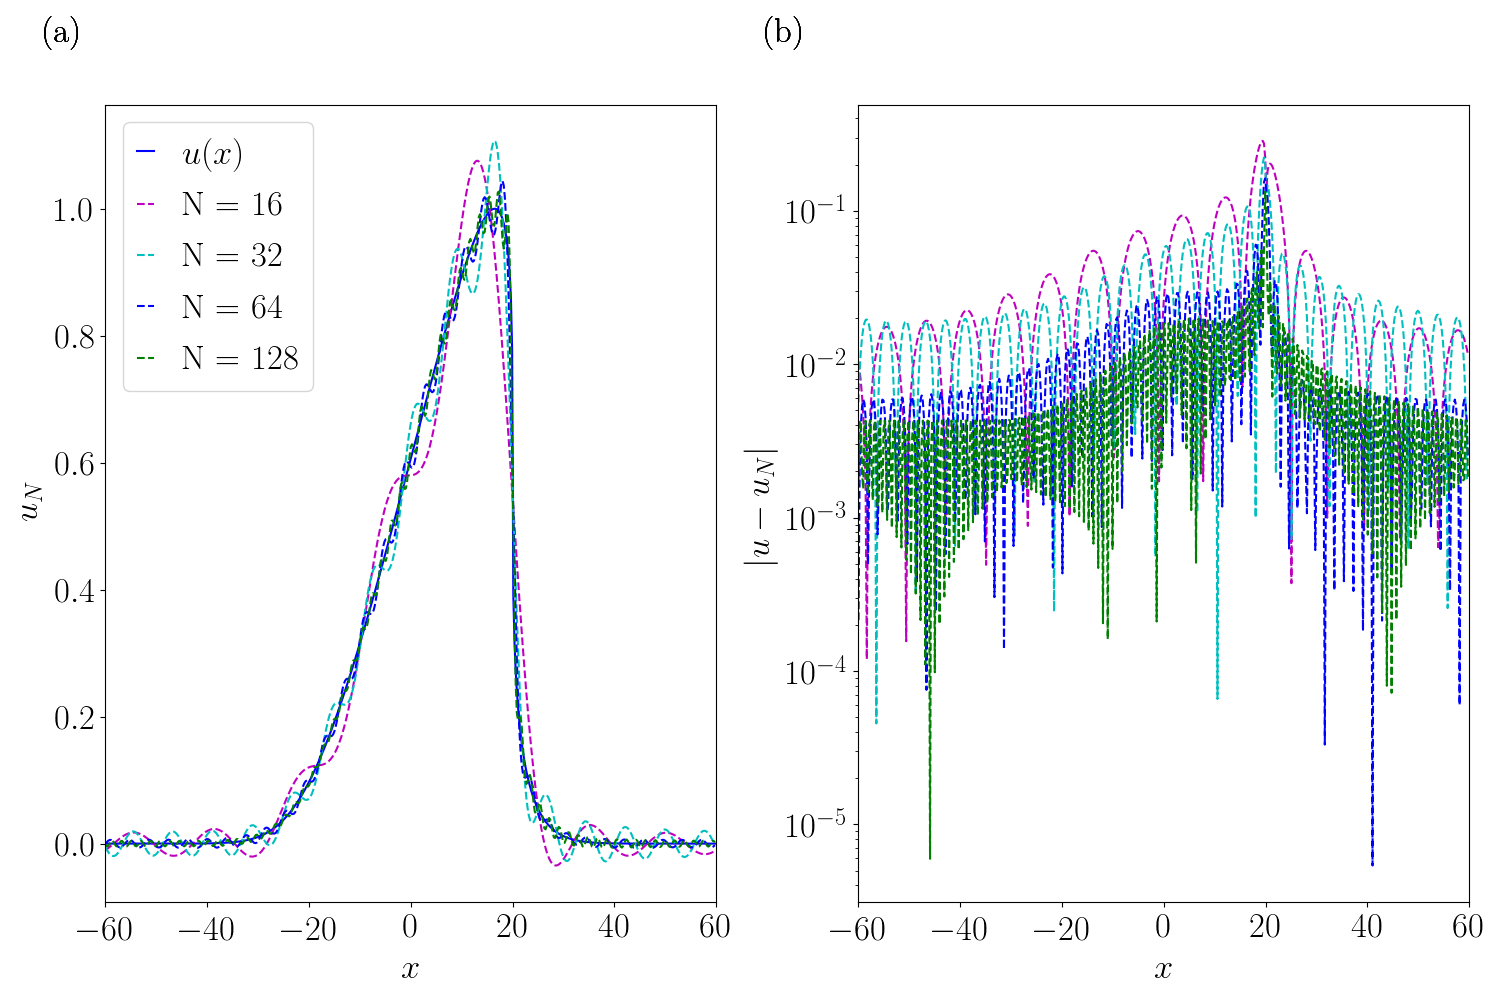
\includegraphics[width=13cm]{Figures/Numerical_Solution_Inviscid_T.png}
		\caption{(a) Exact solution for the problem defined in the example (\ref{Convection_Well}), and its approximations using the scheme given by (\ref{Convection_scheme}) at the time $Tc$ with initial condition $u_0(x) = e^{-0.005x^2}$, $x \in [-60, 60]$. (b) Pointwise error of approximation.}
		\label{convection_aprox_T}
		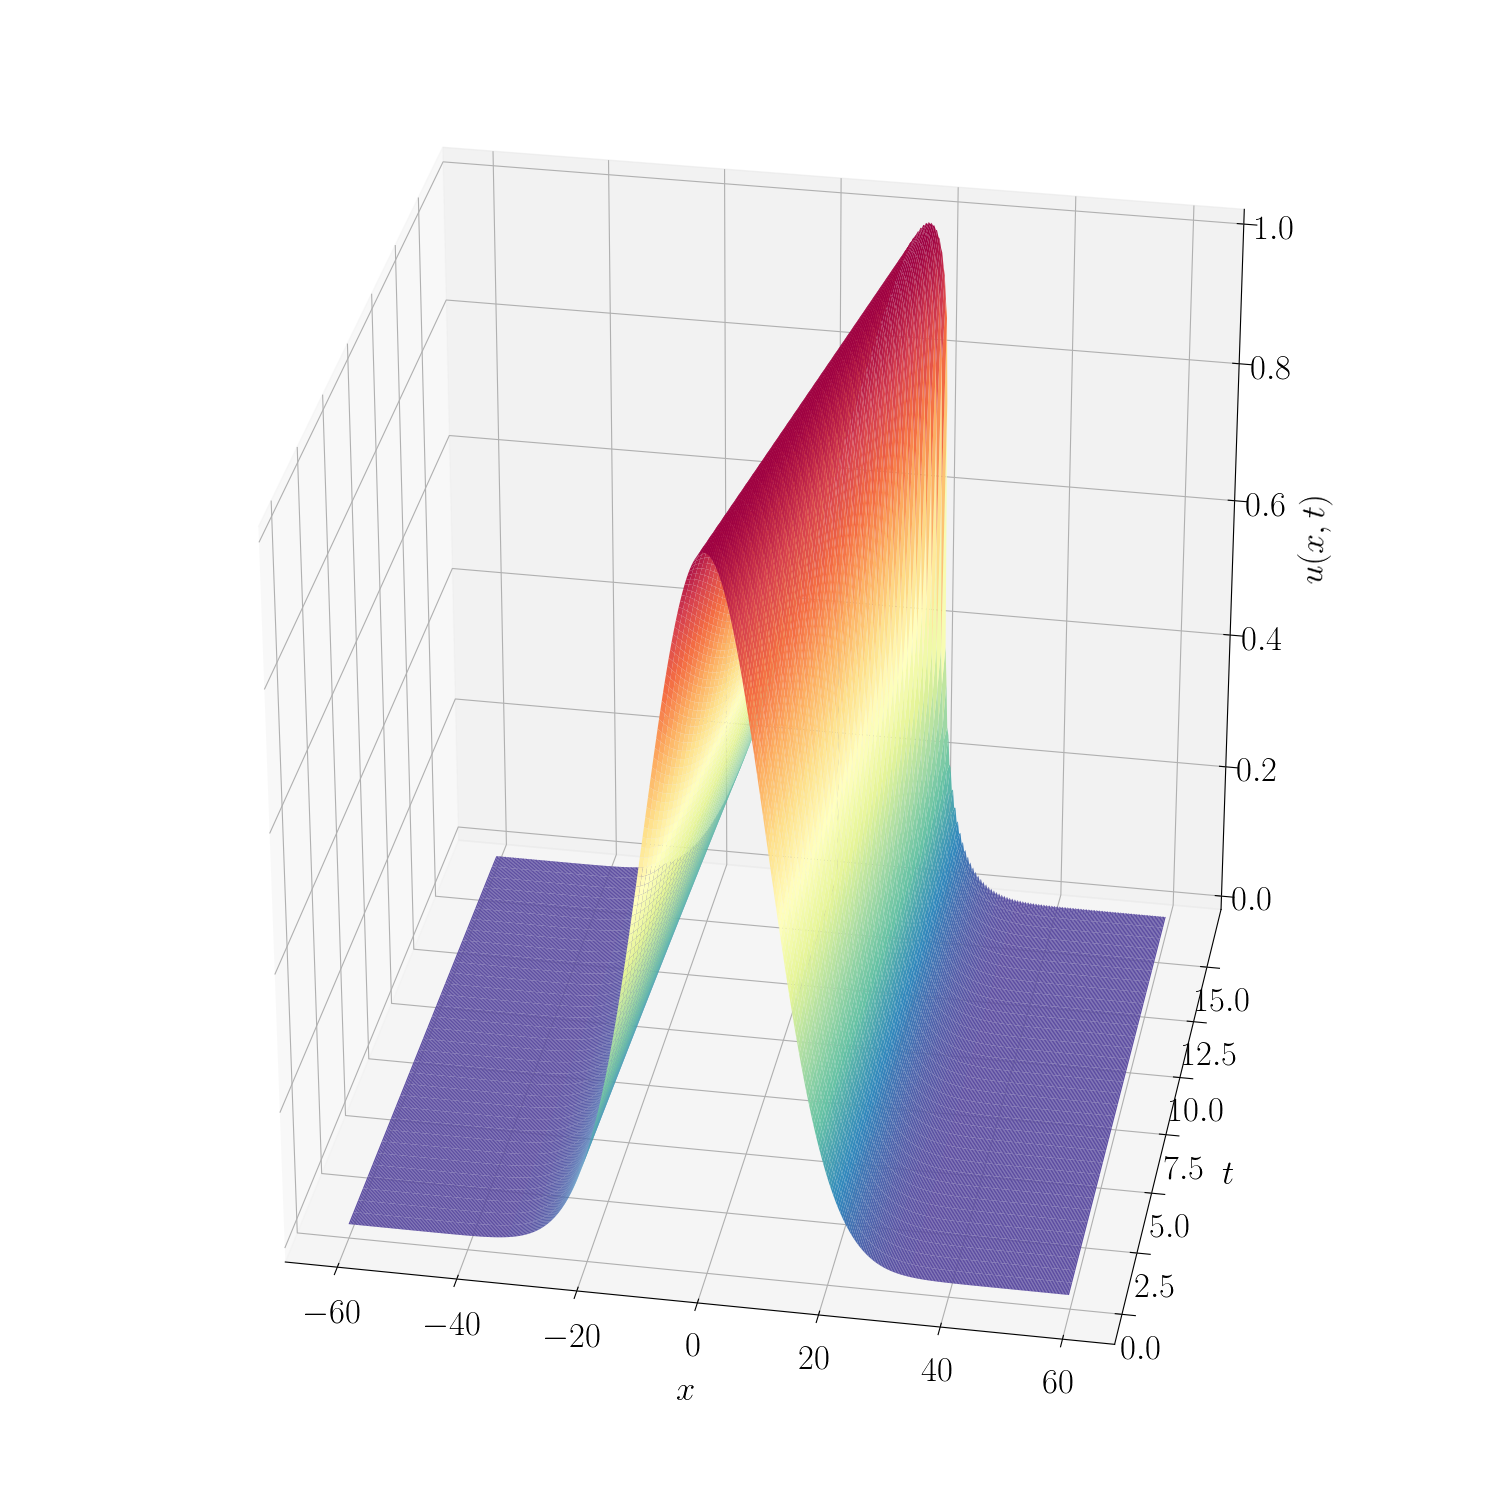
\includegraphics[width=11cm]{Figures/Numerical_Solution_Inviscid.png}
		\caption{Numerical approximation for the problem defined in the Example \ref{Convection_Well} using the scheme given by (\ref{Convection_scheme}) with $N=512$, $u_0(x) = e^{-0.005x^2}$, $x \in [-60, 60]$, and $t \in [0, Tc]$.}
	\end{figure}
	
	As before, we will discretize the time variable $t$ over the interval $[0, T_c]$, where $T_c$ is given as in (\ref{shock_time}), as follows
	\begin{align*}
		t_i = i \Delta t, \hspace{2mm} i = 0, 1, \dots, T_c
	\end{align*}
	
	Recall that the solution for (\ref{Inviscid}) is given by the characteristic curves as follows
	\begin{align}
		u(x, t) = u_0 (x_0), \hspace{2mm} x_0 = x - u_0 (x_0) t, 
	\end{align}
	which is resolved for every $t$ and every $x_0 \in [x_L, x_R]$. \\
	
	In the following simulations, the Galerkin method given by (\ref{full_discrete}) was used to obtain numerical solutions with small values of $\alpha$ and compare them with the exact solution given above corresponding to the problem without viscosity.
	
	\begin{figure}[H]
		\centering
		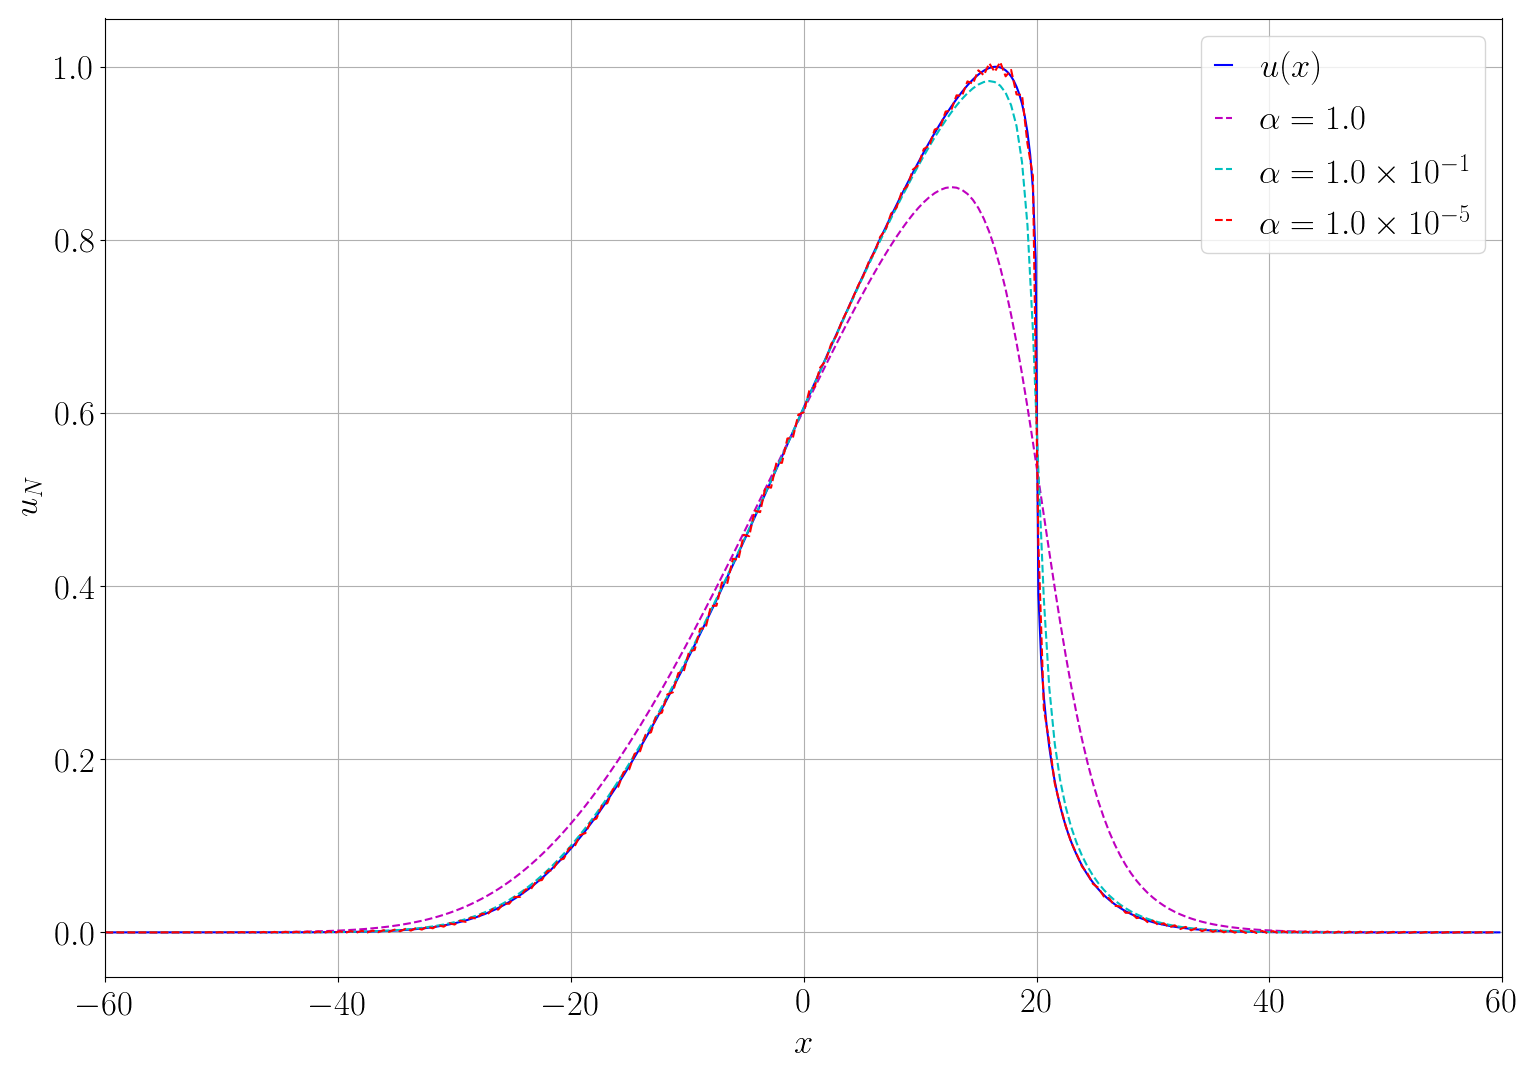
\includegraphics[width=12cm]{Figures/varios_alphas.png}
		\caption{Exact solution for (\ref{Inviscid}) and different approximations using (\ref{full_discrete}) with $N=256$, and $\Delta t = 1.0 \times 10^{-3}$.}
	\end{figure}
	\newpage
	\begin{figure}[H]
		\centering
		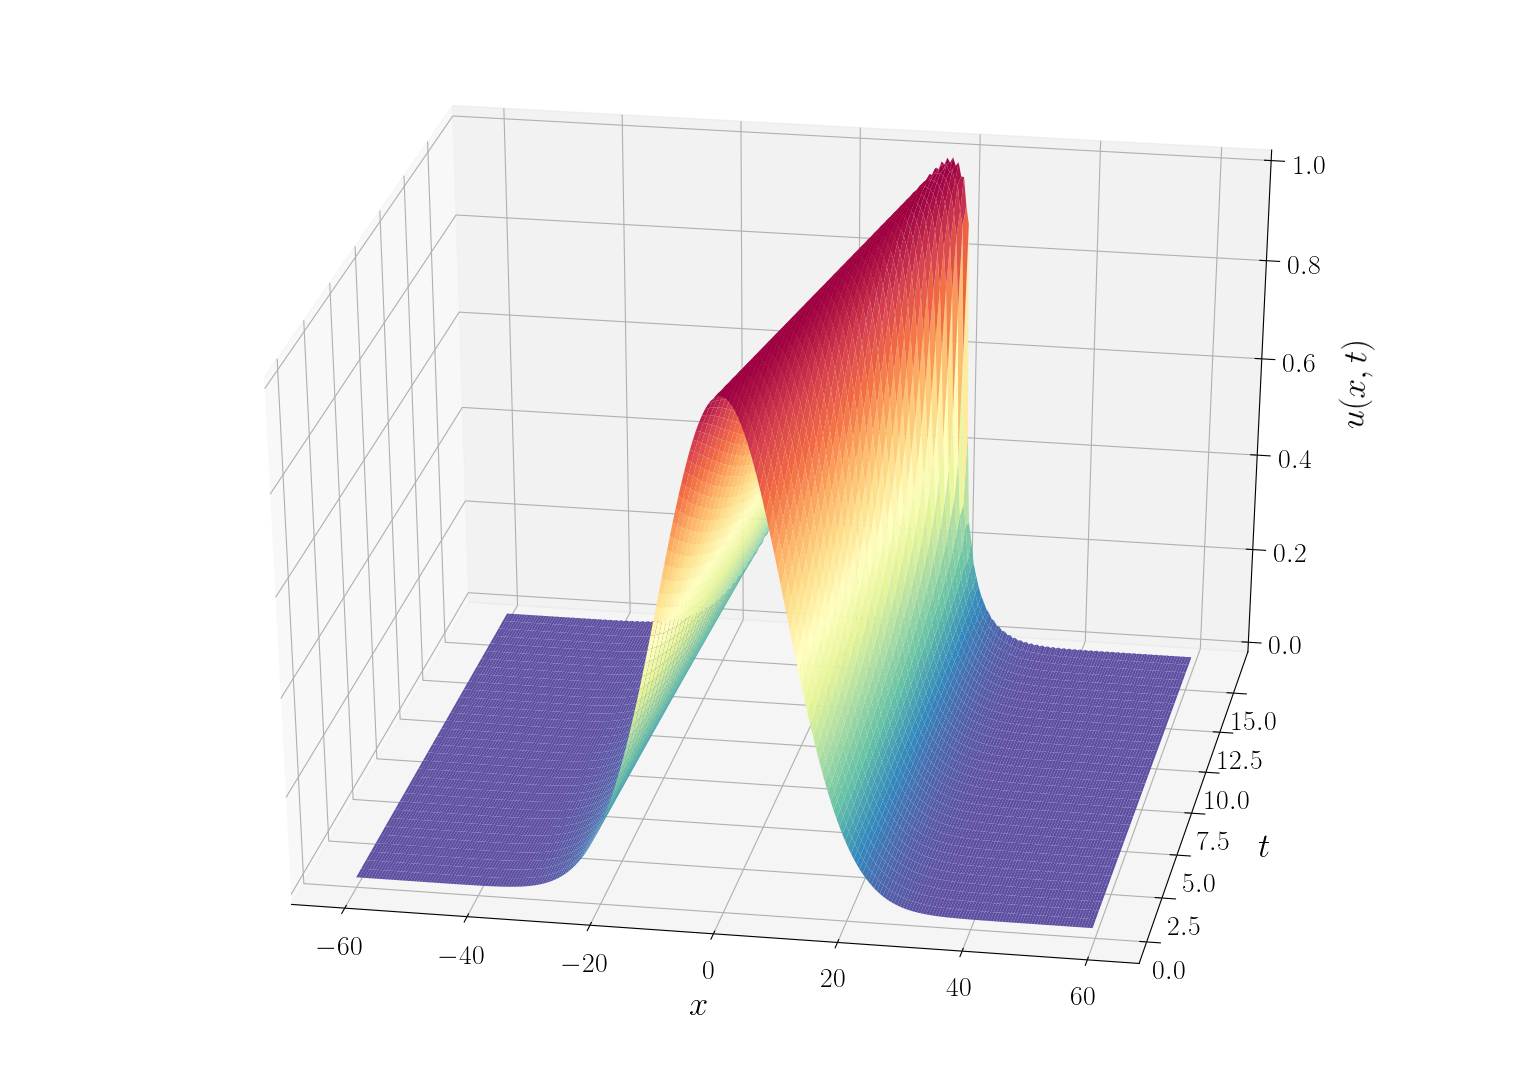
\includegraphics[width=12cm]{Figures/small_alpha.png}
		\caption{Numerical solution for (\ref{burgers}) using (\ref{full_discrete}) with $\alpha = 1.0 \times 10^{-5}$, $N=256$, and $\Delta t = 1.0 \times 10^{-3}$.}
		\vspace{2mm}
		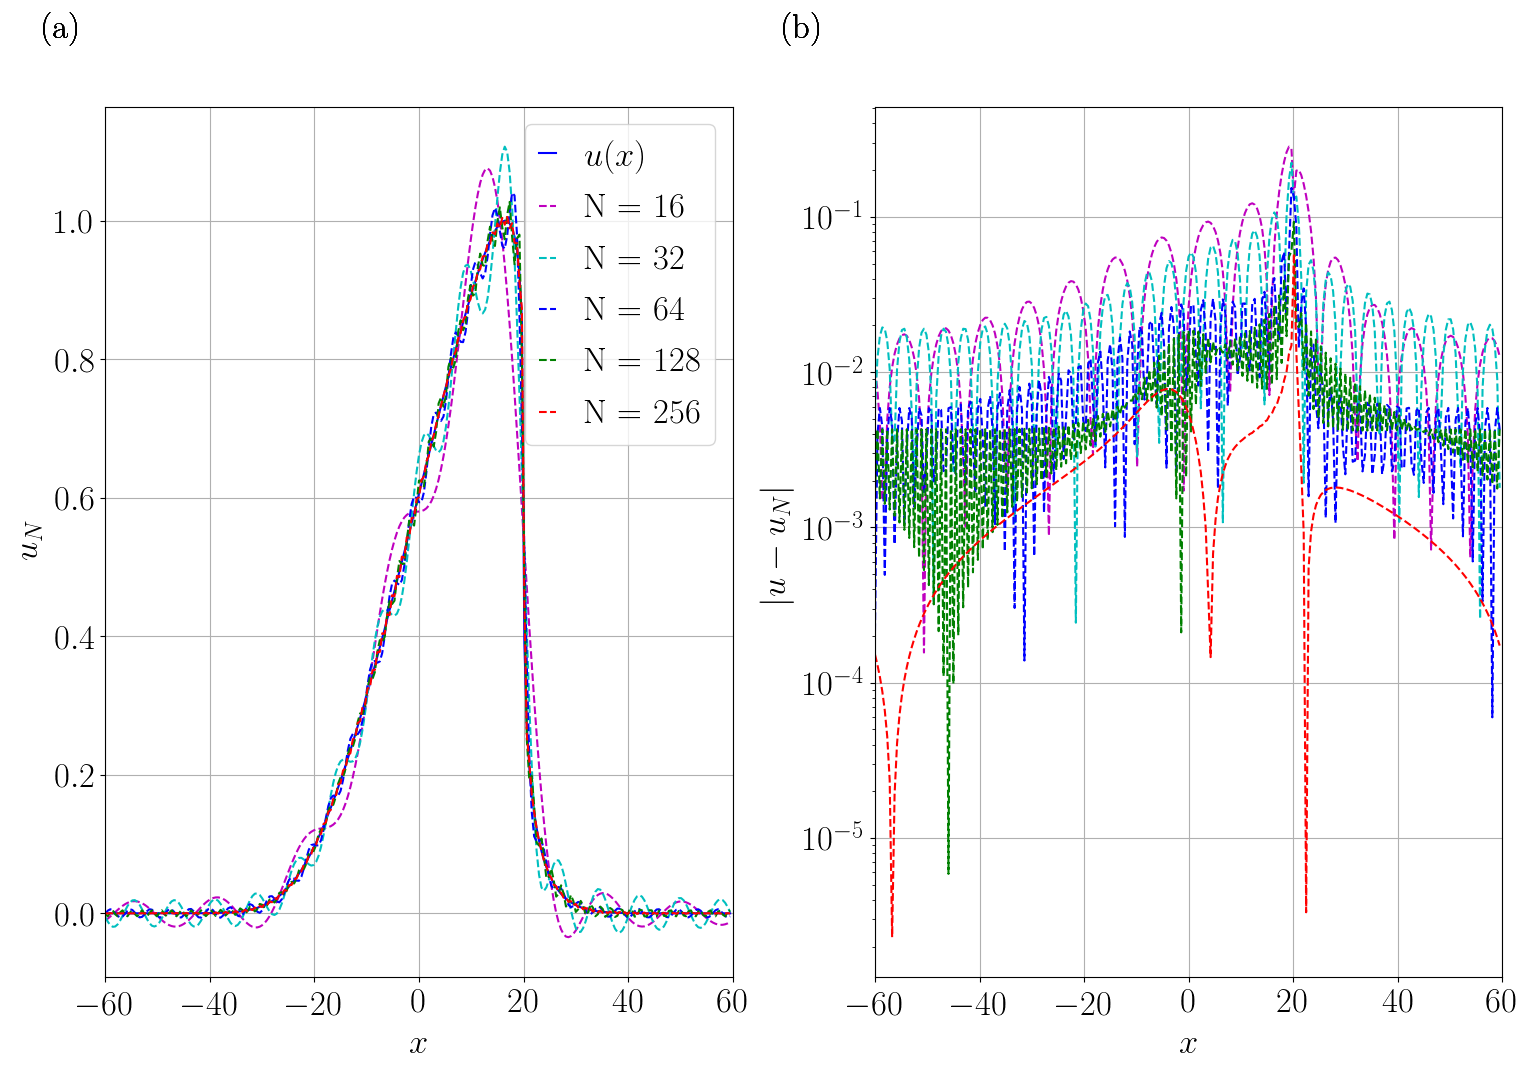
\includegraphics[width=12.5cm]{Figures/small_alpha_T.png}
		\caption{Numerical solution for (\ref{burgers}) using (\ref{full_discrete}) at the time $T_c$ with $\alpha = 1.0 \times 10^{-5}$, and $\Delta t = 1.0 \times 10^{-3}$. (b) Point-wise error of approximation.}
	\end{figure}
	\begin{table}[H]
		\centering
		\begin{tabular}{lccc}
			\toprule
			\multicolumn{1}{c}{\textbf{Approximation}} & \multicolumn{3}{c}{\textbf{Distance}} \\
			\hspace{12mm} $N$ & $\Delta t=1\times 10^{-2}$ & $\Delta t=1\times 10^{-3}$ & $\Delta t=1\times 10^{-4}$ \\
			\midrule
			\hspace{12mm} 16 & 0.285531 & 0.285732 & 0.285752 \\
			\midrule
			\hspace{12mm} 32 & 0.222737 & 0.223260 & 0.223312 \\
			\midrule
			\hspace{12mm} 64 & 0.160385 & 0.162782 & 0.163025 \\
			\midrule
			\hspace{12mm} 128 & 0.129297 & 0.133322 & 0.133733 \\
			\midrule
			\hspace{12mm} 256 & 0.083291 & 0.091449 & 0.092320 \\
			\bottomrule
		\end{tabular}
		\caption{Distance between exact solution for (\ref{Inviscid}) and the approximation for (\ref{burgers}) with $\alpha = 1.0 \times 10^{-5}$.}
	\end{table}